\section{El proyecto funcionando en Docker}
Para que nuestro poyecto inicie primero iniciamos nuestro contenedor previamente creado :
\begin{figure}[H]
  \centering
  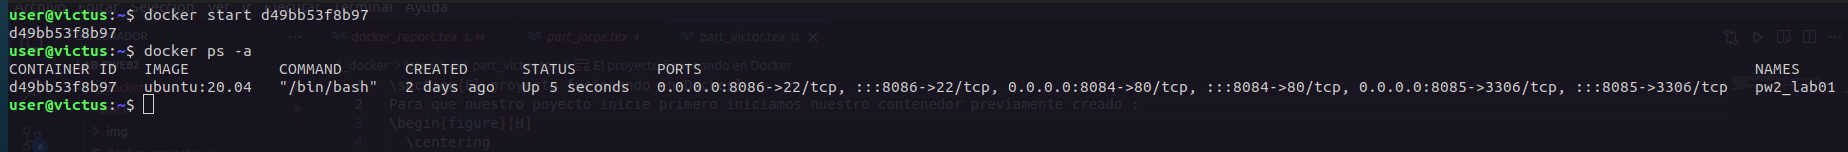
\includegraphics[width=1.0\textwidth]{img/Iniciando_Docker.png}
  \caption{Poner en funcionamiento el contenedor Docker}
\end{figure}
Iniciamos los servicios Apache 2, MySQL y OpenSSH en un contenedor Docker. Los comandos primero iniciamos el contenedor 
\begin{verbatim}
  docker exec -it pw2_lab01 /bin/bash 
\end{verbatim}
\hspace{0.5cm}Despues de acceder al contenedor, y luego se inician los servicios con los comandos correspondientes 
(\textit{apache2 start}, \textit{mysql start}, \textit{ssh start}).
\begin{figure}[H]
  \centering
  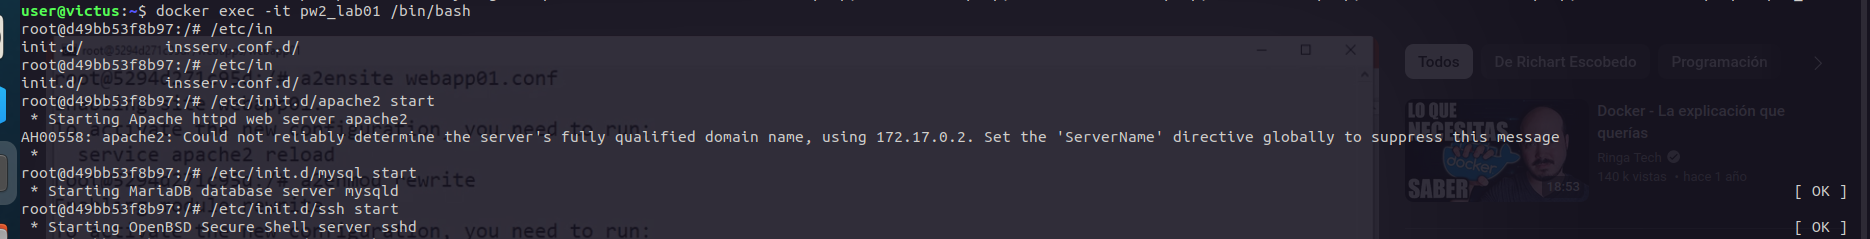
\includegraphics[width=1.0\textwidth]{img/Activamos_servicios.png}
  \caption{Entrando al contenedor Docker y activando servicios}
\end{figure}


Creamos la carpeta donde se encontraran nuestras aplicaciones web. La cual se se llamara aplicaciones-web y dentro de esta pondremos el 
proyecto final pweb1 la cual fue desarrollada en la rama styles para su uso 
\begin{figure}[H]
  \centering
  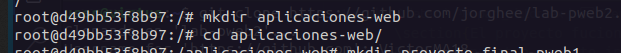
\includegraphics[width=1.0\textwidth]{img/Creamos_carpeta.png}
  \caption{Creamos la carpeta para las aplicaciones web}
\end{figure}
\begin{figure}[H]
  \centering
  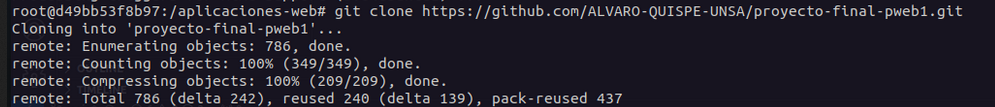
\includegraphics[width=1.0\textwidth]{img/Clonamos_proyecto.png}
  \caption{clonamos el proyecto en la carpeta de las aplicaciones web}
\end{figure}
\begin{figure}[H]
  \centering
  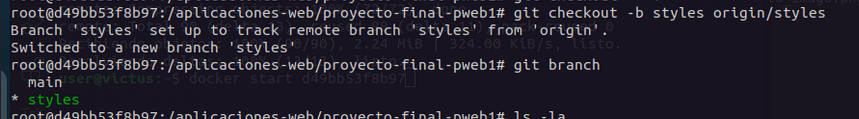
\includegraphics[width=1.0\textwidth]{img/Cambiando_Rama.png}
  \caption{Cambiamos de rama proyecto en la carpeta de las aplicaciones web}
\end{figure}

Tambien creamos una configuracion del directorio en virtualhost y tambien su alias para eso hacemos un archivo .conf dentro de la carpeta 
/etc/apache2/sites-available/proyecto-final-pweb1.conf para esto tambien activamos la configuracion con a2ensite, a2enmod y reiniciamos el servidor apache
\begin{figure}[H]
  \centering
  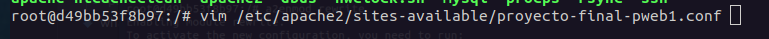
\includegraphics[width=1.0\textwidth]{img/Creacion_conf.png}
  \caption{Creamos la configuracion de la carpeta para que pueda funcionar con apache}
\end{figure}
\begin{figure}[H]
  \centering
  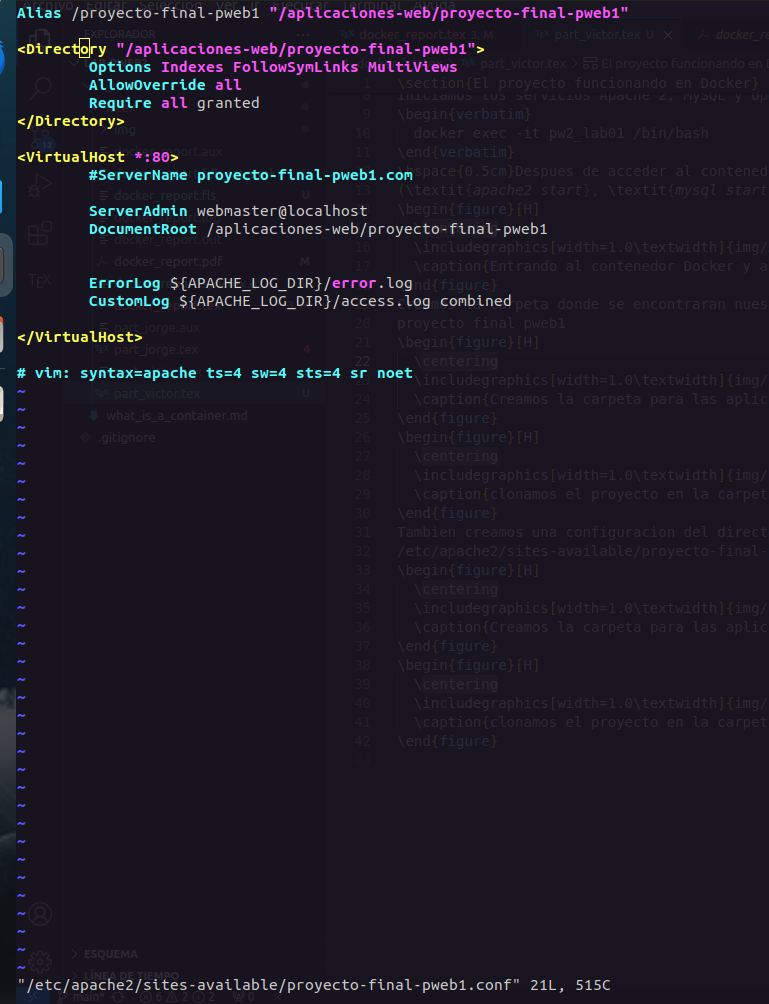
\includegraphics[width=1.0\textwidth]{img/Configuracion.png}
  \caption{Creamos la configuracion de la carpeta para que pueda funcionar con apache}
\end{figure}
\begin{figure}[H]
  \centering
  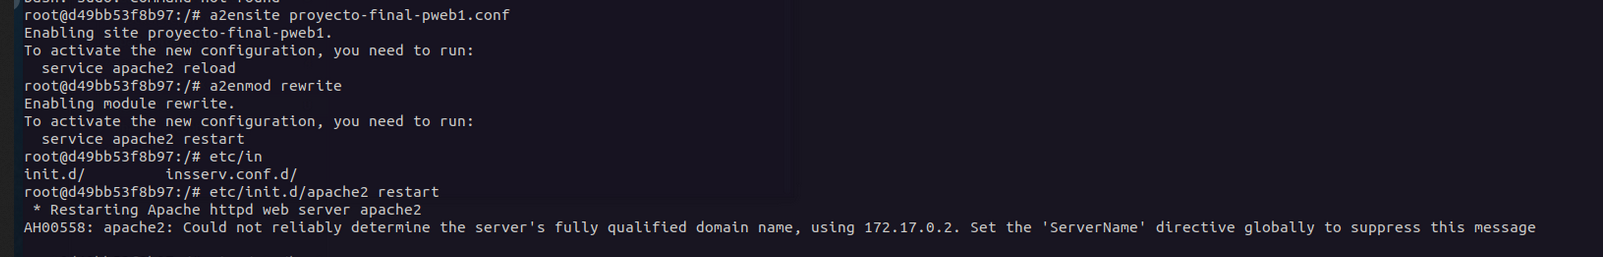
\includegraphics[width=1.0\textwidth]{img/Activacion_configuracion.png}
  \caption{Activamos la configuracion y reiniciamos apache}
\end{figure}
Tambien activamos los accesos para el servidor en /etc/hosts para nuestro proyecto en el ordenador para los ip's  
\begin{figure}[H]
  \centering
  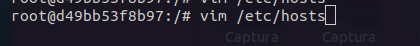
\includegraphics[width=1.0\textwidth]{img/Carpeta_hosts.png}
  \caption{Vamos a la configuracion de los hosts}
\end{figure}
\begin{figure}[H]
  \centering
  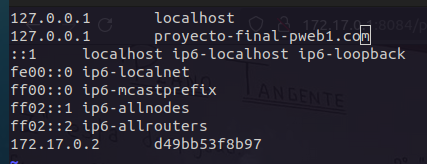
\includegraphics[width=1.0\textwidth]{img/Config_hosts.png}
  \caption{Vamos a la configuracion de los hosts}
\end{figure}

Despues tambien creamos nuestro usuario pw2 con la contraseña 12345678 la cual va tener permisos de nuestro proyecto tambien instalaremos, apt-get install perl
a2enmod cgid, apt-get install libapache2-mod-fcgid para poder usar los archivos .pl para esto tambien hacemos una configuracion en /etc/apache2/conf-available - vim cgi-bin.conf
donde habilitaremos la ejecucicion de los .pl de nuestro proyecto
\begin{figure}[H]
  \centering
  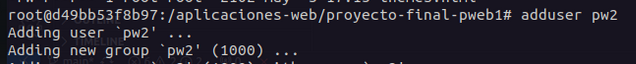
\includegraphics[width=1.0\textwidth]{img/Usuario_pw2.png}
  \caption{Creacion del usuario}
\end{figure}
\begin{figure}[H]
  \centering
  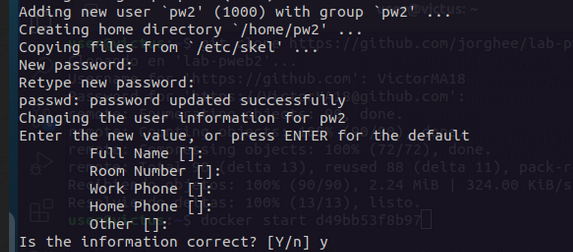
\includegraphics[width=1.0\textwidth]{img/Usuario_pw2_2.png}
  \caption{Creacion del usuario}
\end{figure}
\begin{figure}[H]
  \centering
  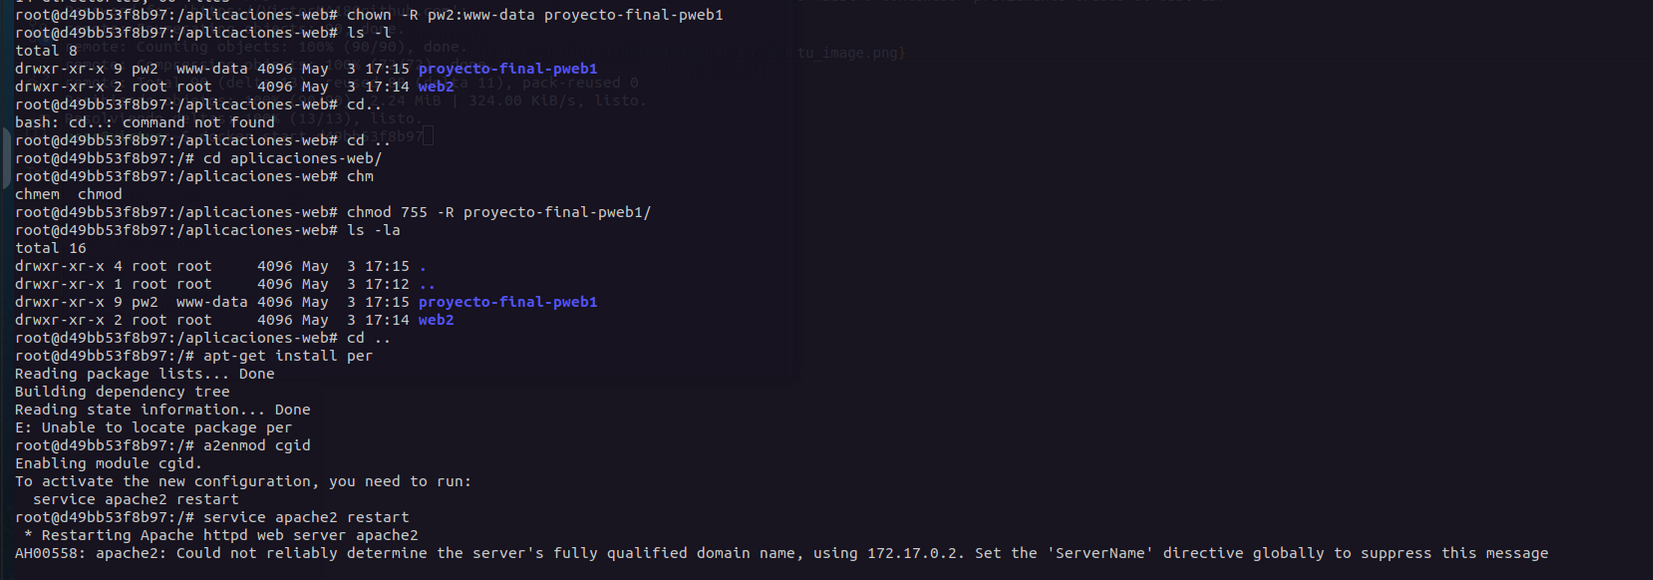
\includegraphics[width=1.0\textwidth]{img/Dando_permisos.png}
  \caption{Dando permisos al ususario pw2}
\end{figure}
\begin{figure}[H]
  \centering
  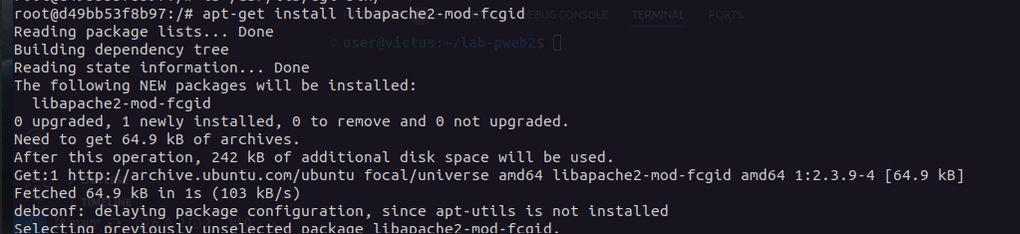
\includegraphics[width=1.0\textwidth]{img/LIbrerias.png}
  \caption{Añadiendo las librerias para el cgi}
\end{figure}
\begin{figure}[H]
  \centering
  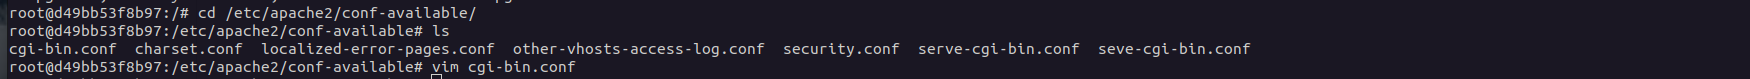
\includegraphics[width=1.0\textwidth]{img/Ubicacion_ejecucion.png}
  \caption{Ubicacion para la ejecucion de los .pl}
\end{figure}
\begin{figure}[H]
  \centering
  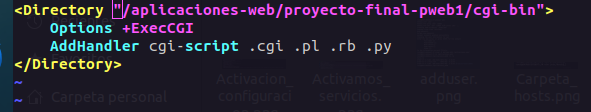
\includegraphics[width=1.0\textwidth]{img/Configurando.png}
  \caption{Configurando el directorio para ejecucion de los archivos.pl}
\end{figure}

Entonces para el siguiente paso seria instalar los modulos de Perl los cuales necesitan primero instalar el paquete make el cual nos va a poder permitir descargar 
los diferentes modulos de Perl los cuales son : CGI::Session; DBI; JSON; DBI:MariaDB para este ultimo se necesitan librerias las cuales son mariadb-client y build-essential
\begin{figure}[H]
  \centering
  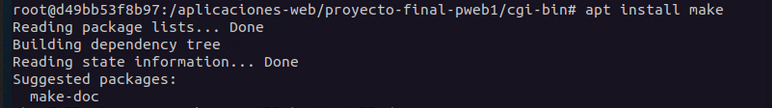
\includegraphics[width=1.0\textwidth]{img/Instalar_make.png}
  \caption{Instalamos el repositorio make para nuestros modulos de perl}
\end{figure}
\begin{figure}[H]
  \centering
  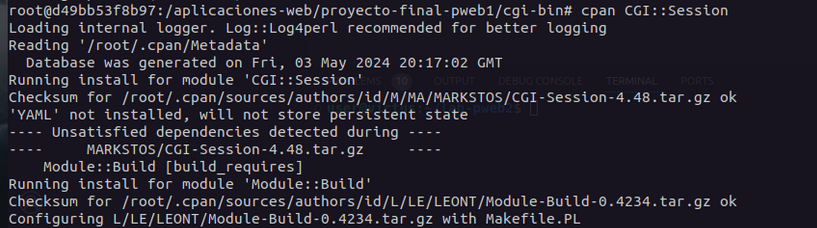
\includegraphics[width=1.0\textwidth]{img/Instalando CGI_Session.png}
  \caption{Instalamos CGi-Session}
\end{figure}
\begin{figure}[H]
  \centering
  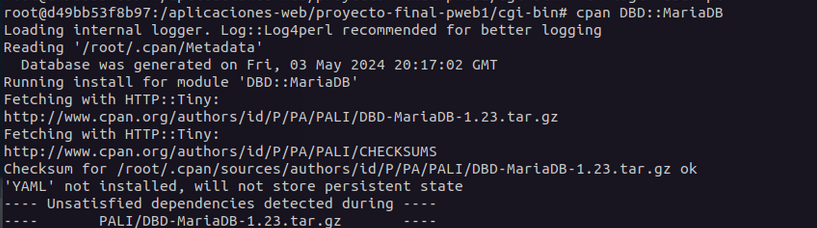
\includegraphics[width=1.0\textwidth]{img/Instalando CGI_MariaDB.png}
  \caption{Instalamos CGI-MariaDB}
\end{figure}
\begin{figure}[H]
  \centering
  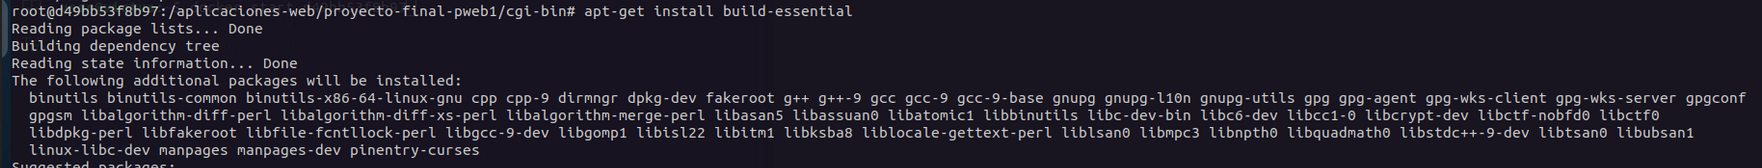
\includegraphics[width=1.0\textwidth]{img/Driver_MariaDB.png}
  \caption{Instalamos los drivers para el funcionamiento de CGI-MariaDB}
\end{figure}
\begin{figure}[H]
  \centering
  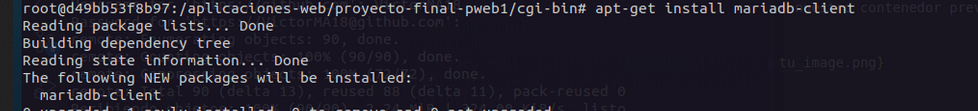
\includegraphics[width=1.0\textwidth]{img/Driver_MariaDB_2.png}
  \caption{Instalamos los drivers para el funcionamiento de CGI-MariaDB}
\end{figure}
\begin{figure}[H]
  \centering
  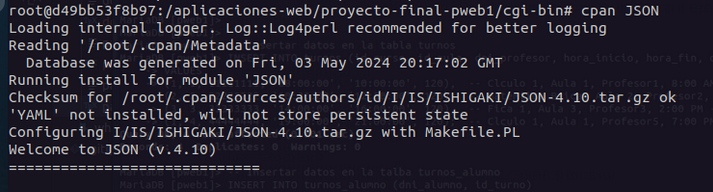
\includegraphics[width=1.0\textwidth]{img/Modulo_JSON.png}
  \caption{Instalamos el modulo JSON para perl}
\end{figure}
\begin{figure}[H]
  \centering
  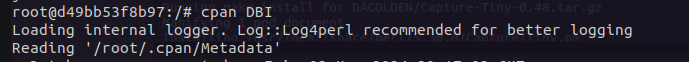
\includegraphics[width=1.0\textwidth]{img/Instalador_DBI.png}
  \caption{Instalamos tambien el modulo DBI}
\end{figure}

En la base de datos insertamos los datos en cada tabla de la base de datos que seria pweb1
\begin{figure}[H]
  \centering
  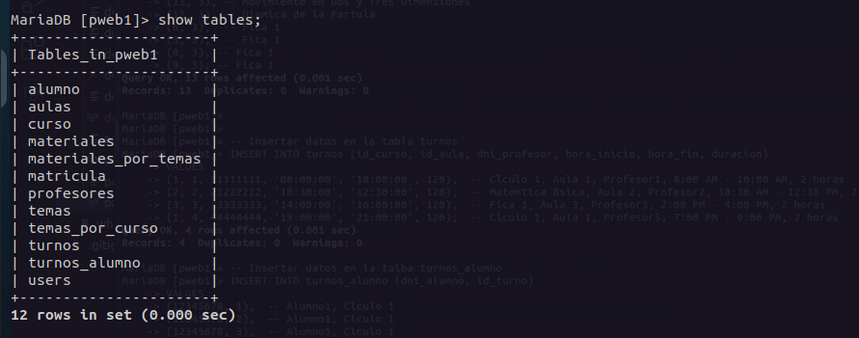
\includegraphics[width=1.0\textwidth]{img/Tablas_pweb1.png}
  \caption{Base de Datos}
\end{figure}
\begin{figure}[H]
  \centering
  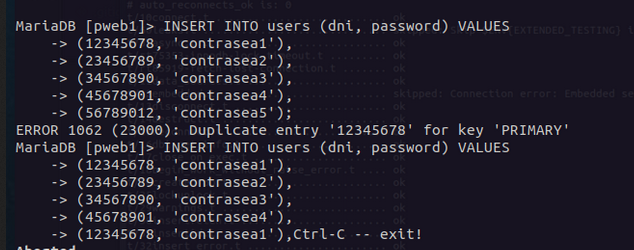
\includegraphics[width=1.0\textwidth]{img/Insertamosdatos_MariaDB.png}
  \caption{Insertando datos en la Base de Datos}
\end{figure}
\begin{figure}[H]
  \centering
  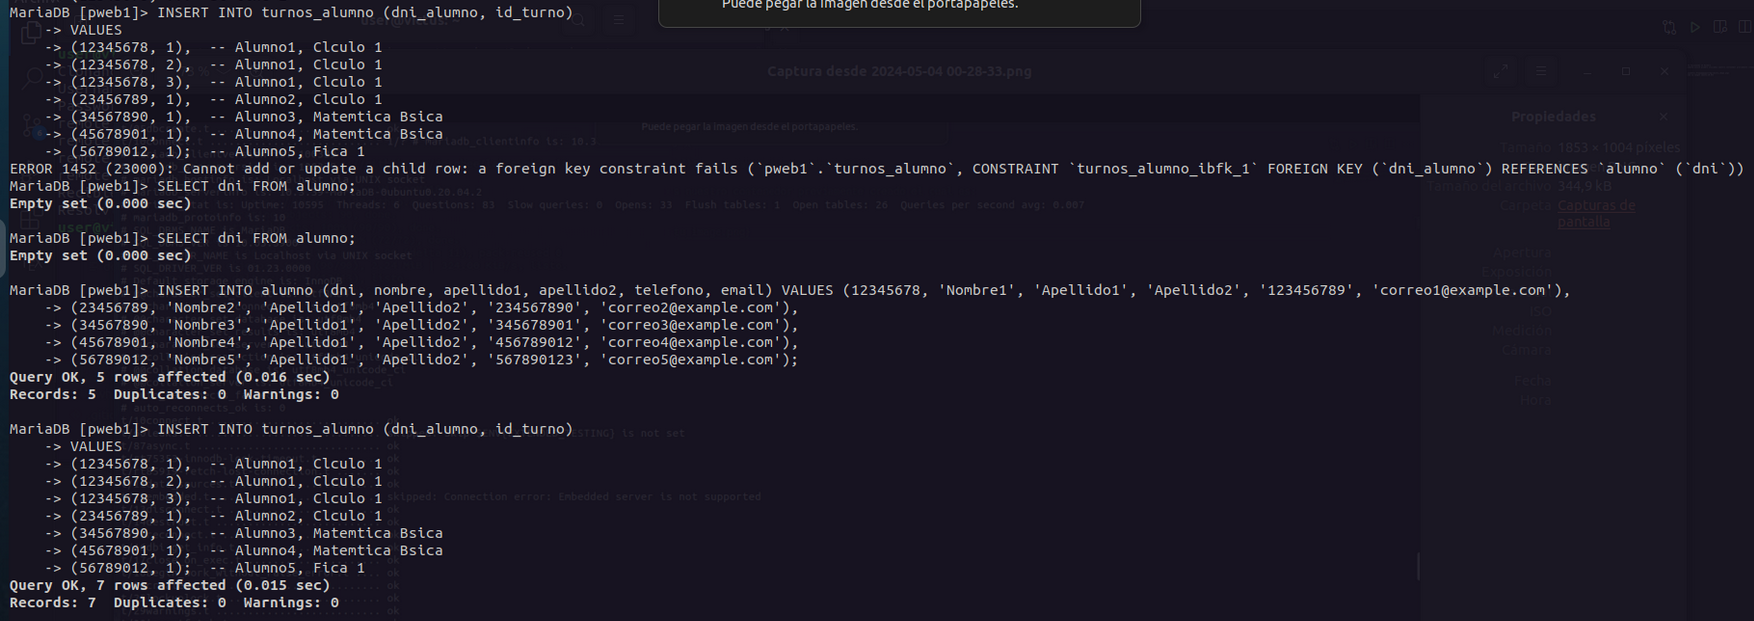
\includegraphics[width=1.0\textwidth]{img/Insertando_Datos_1.png}
  \caption{Insertando datos en la Base de Datos}
\end{figure}
\begin{figure}[H]
  \centering
  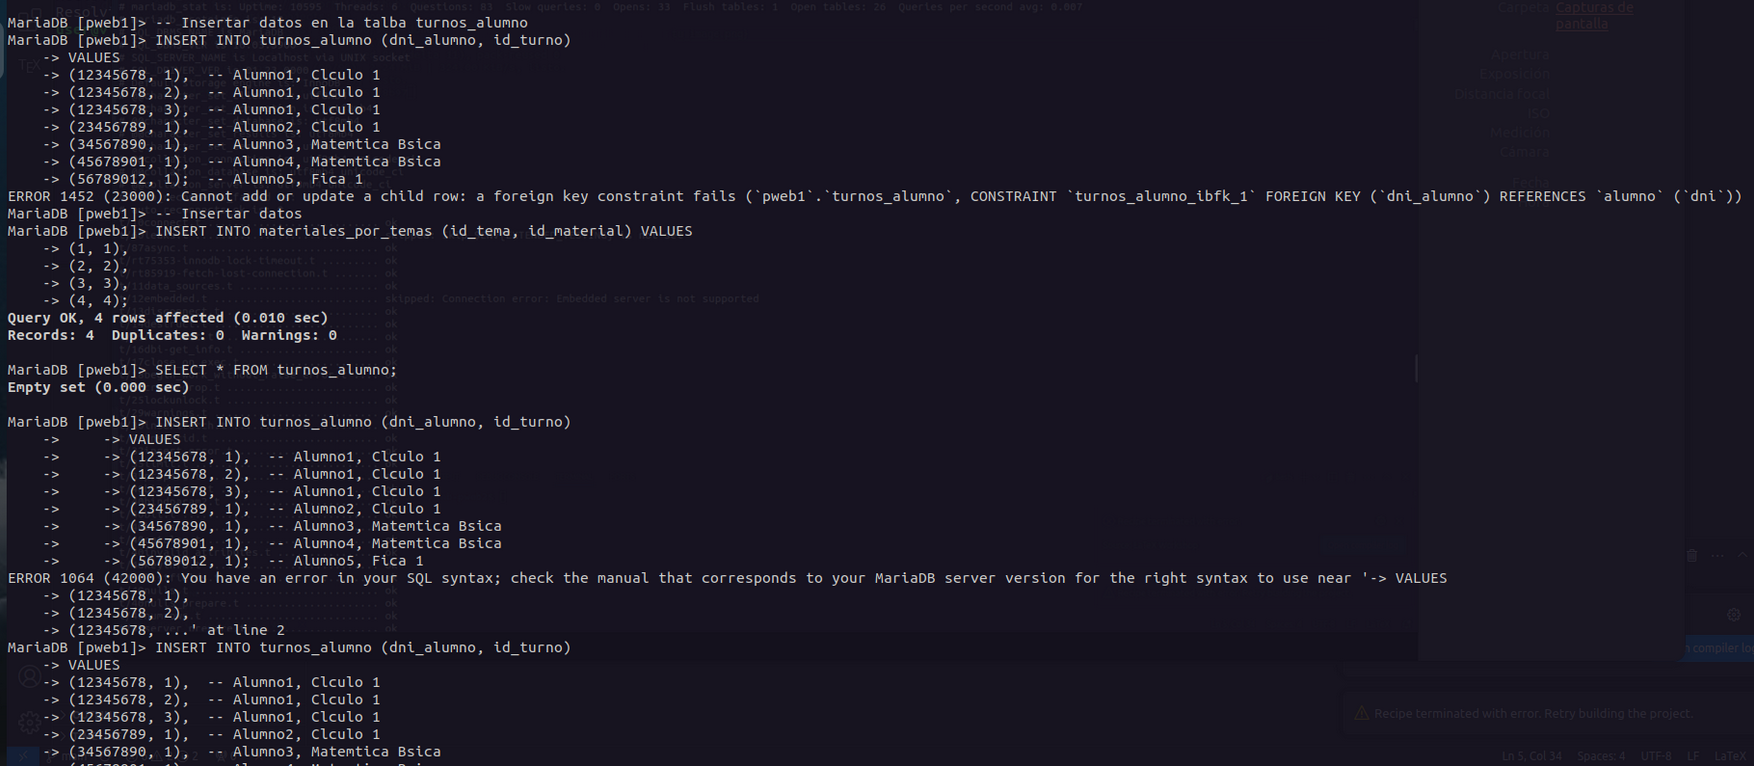
\includegraphics[width=1.0\textwidth]{img/Insertando_Datos_2.png}
  \caption{Insertando datos en la Base de Datos}
\end{figure}
\begin{figure}[H]
  \centering
  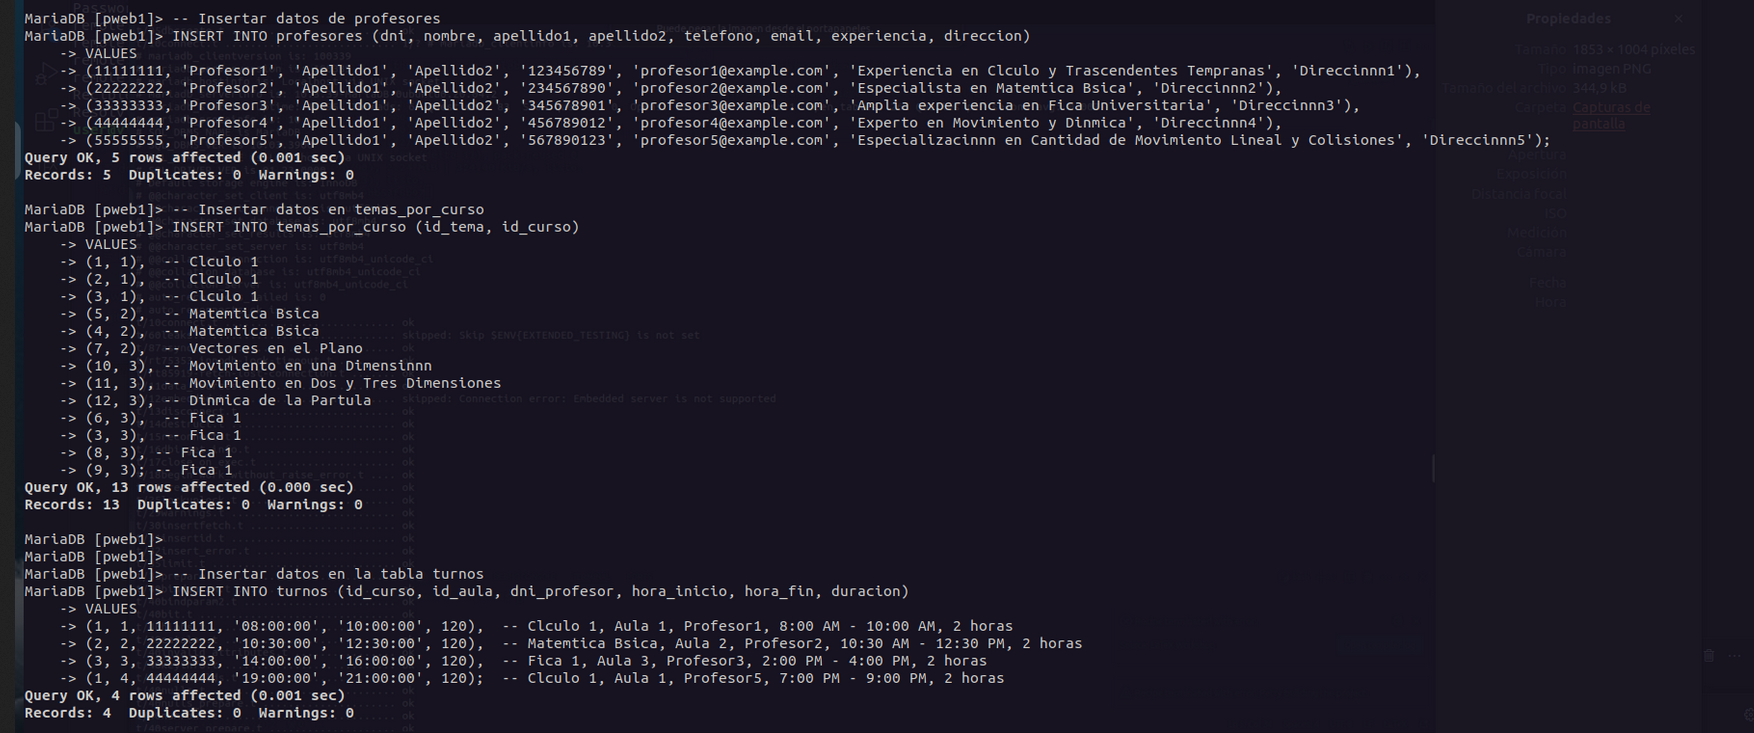
\includegraphics[width=1.0\textwidth]{img/Insertando_Datos_3.png}
  \caption{Insertando datos en la Base de Datos}
\end{figure}
\begin{figure}[H]
  \centering
  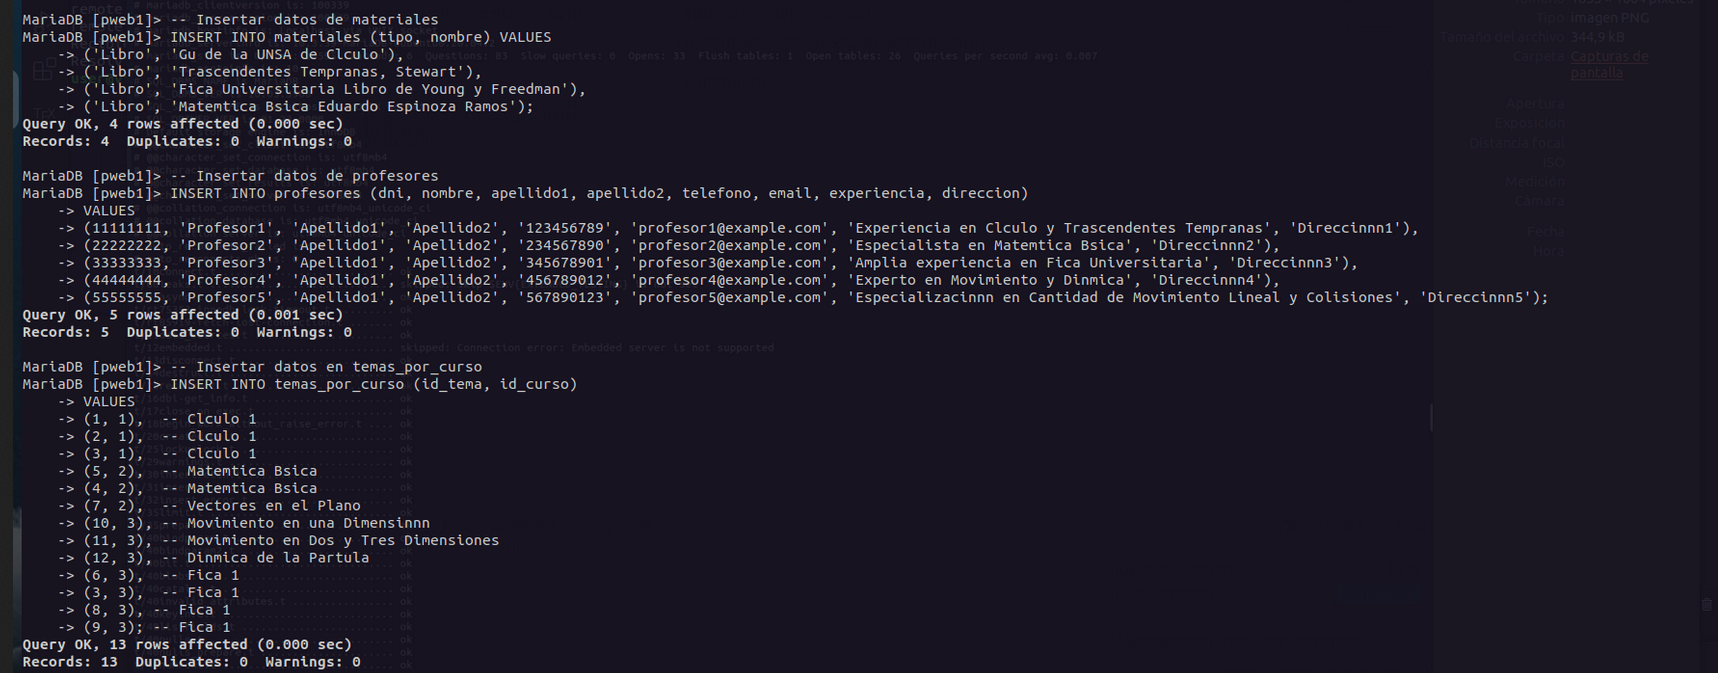
\includegraphics[width=1.0\textwidth]{img/Insertando_Datos_4.png}
  \caption{Insertando datos en la Base de Datos}
\end{figure}
\begin{figure}[H]
  \centering
  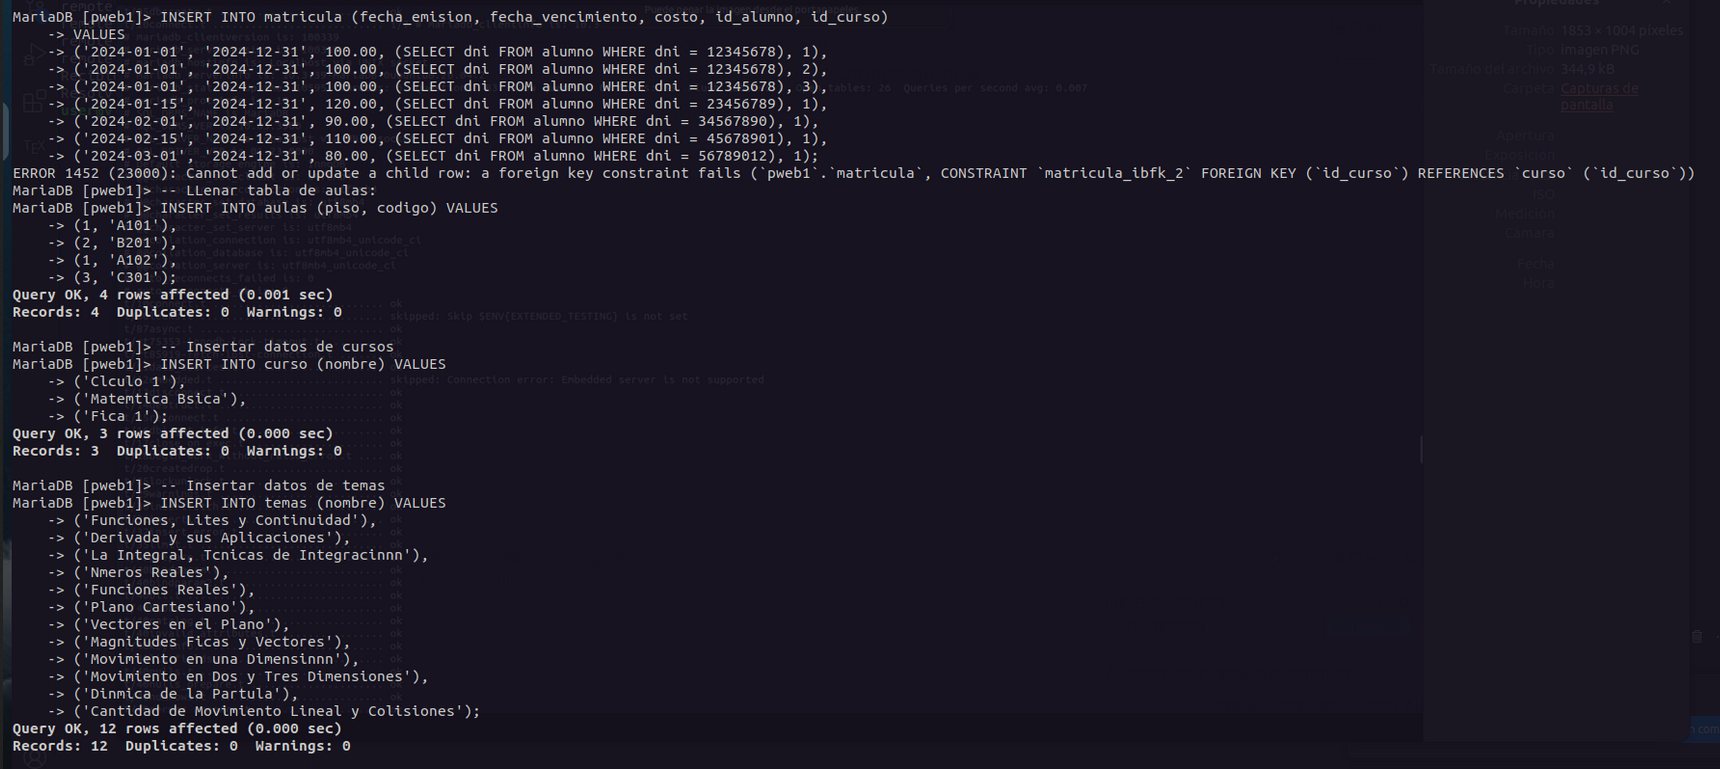
\includegraphics[width=1.0\textwidth]{img/Insertando_Datos_5.png}
  \caption{Insertando datos en la Base de Datos}
\end{figure}

Visualizamos las tablas:
\begin{figure}[H]
  \centering
  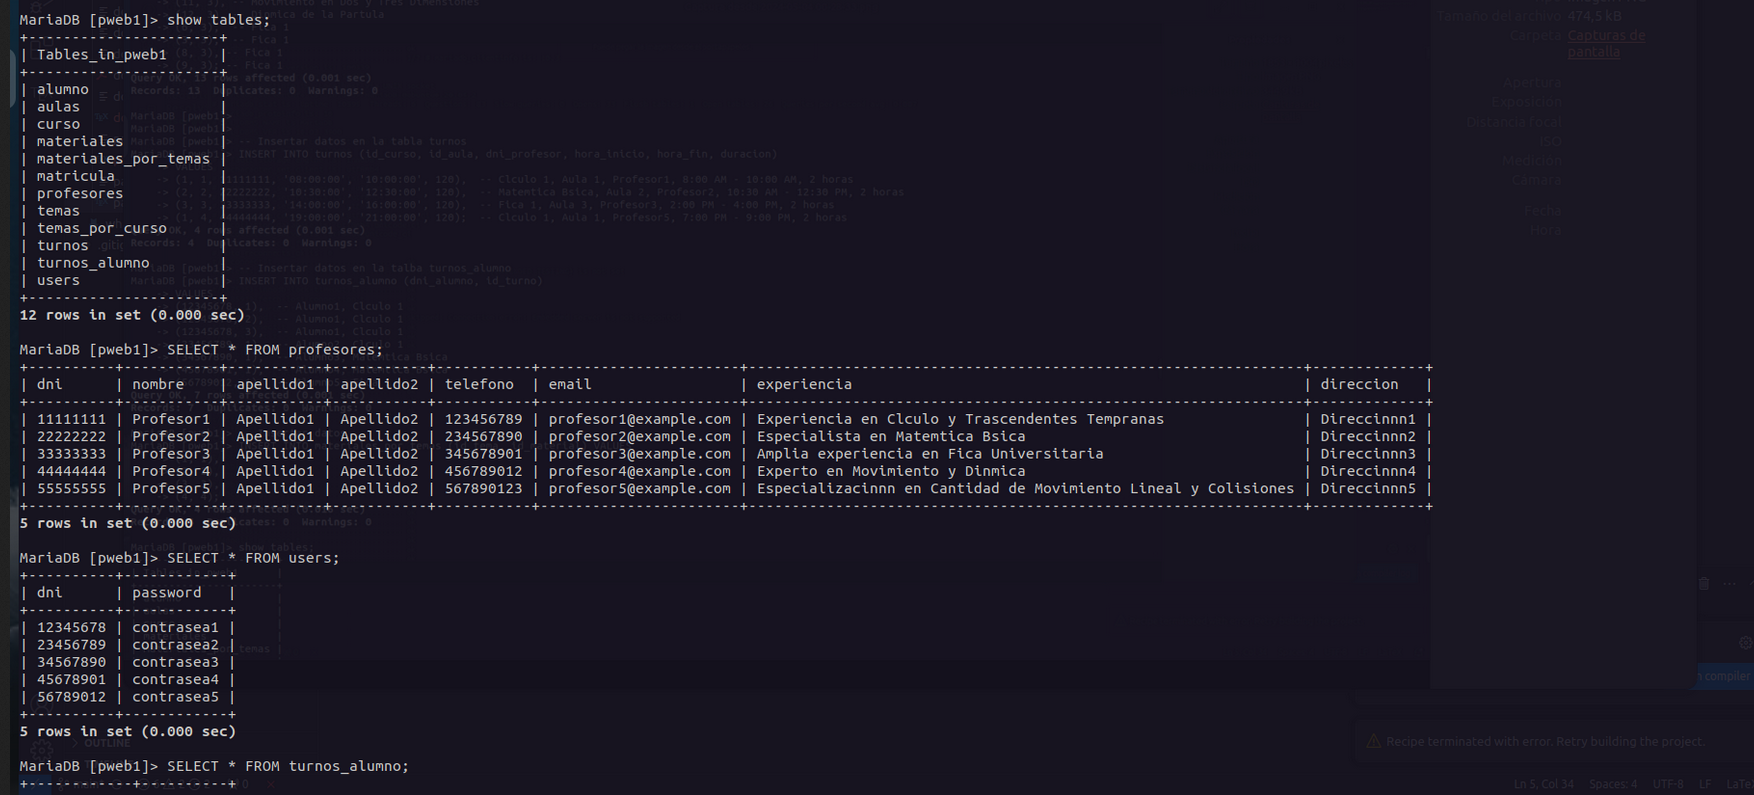
\includegraphics[width=1.0\textwidth]{img/Viendo_Datos_6.png}
  \caption{Visualizamos las tablas de la Base de Datos}
\end{figure}
\begin{figure}[H]
  \centering
  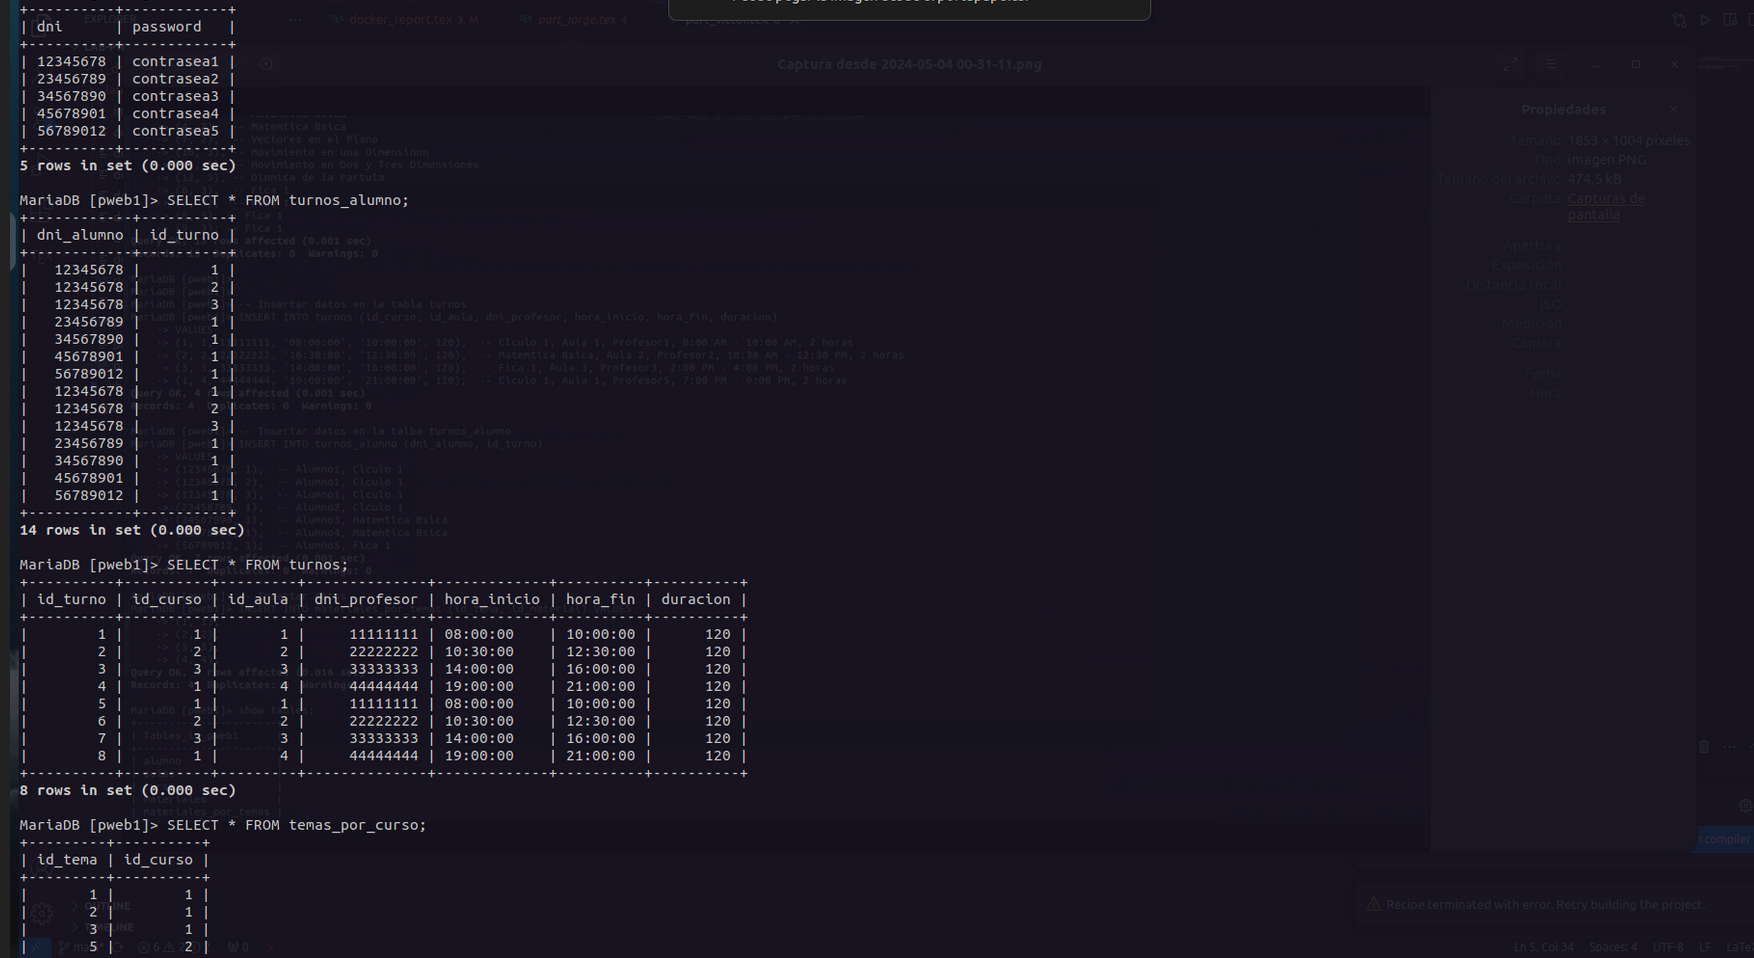
\includegraphics[width=1.0\textwidth]{img/Viendo_Datos_5.png}
  \caption{Visualizamos las tablas de la Base de Datos}
\end{figure}
\begin{figure}[H]
  \centering
  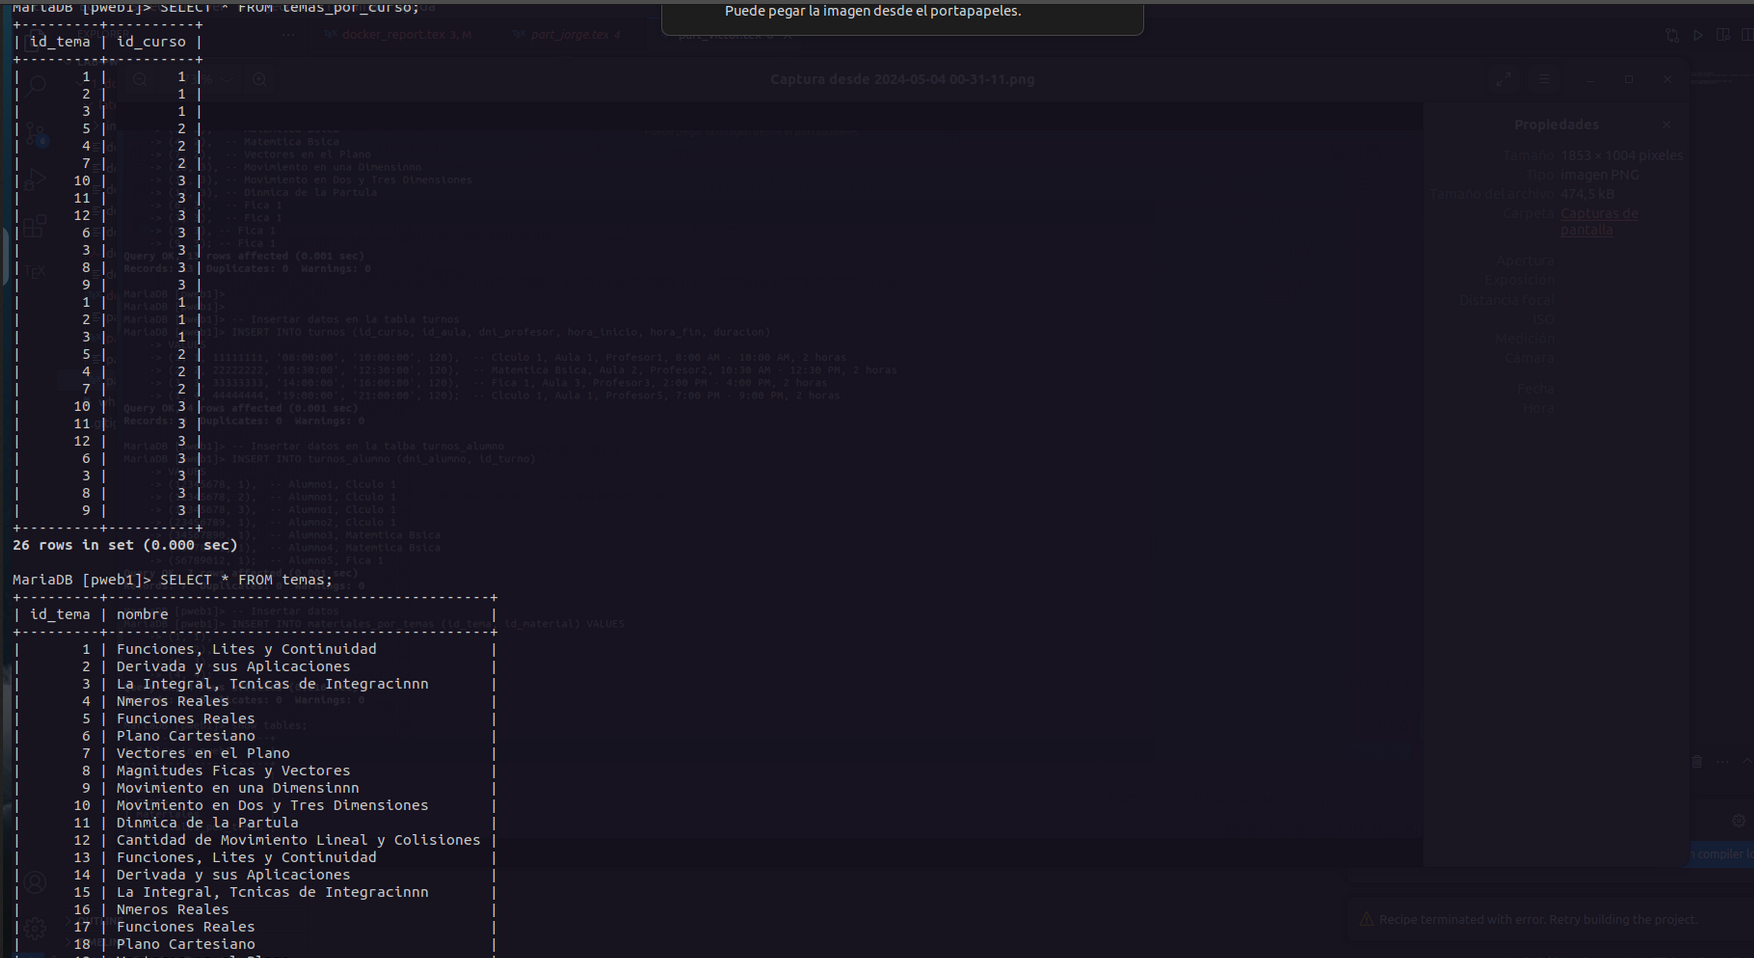
\includegraphics[width=1.0\textwidth]{img/Viendo_Datos_4.png}
  \caption{Visualizamos las tablas de la Base de Datos}
\end{figure}
\begin{figure}[H]
  \centering
  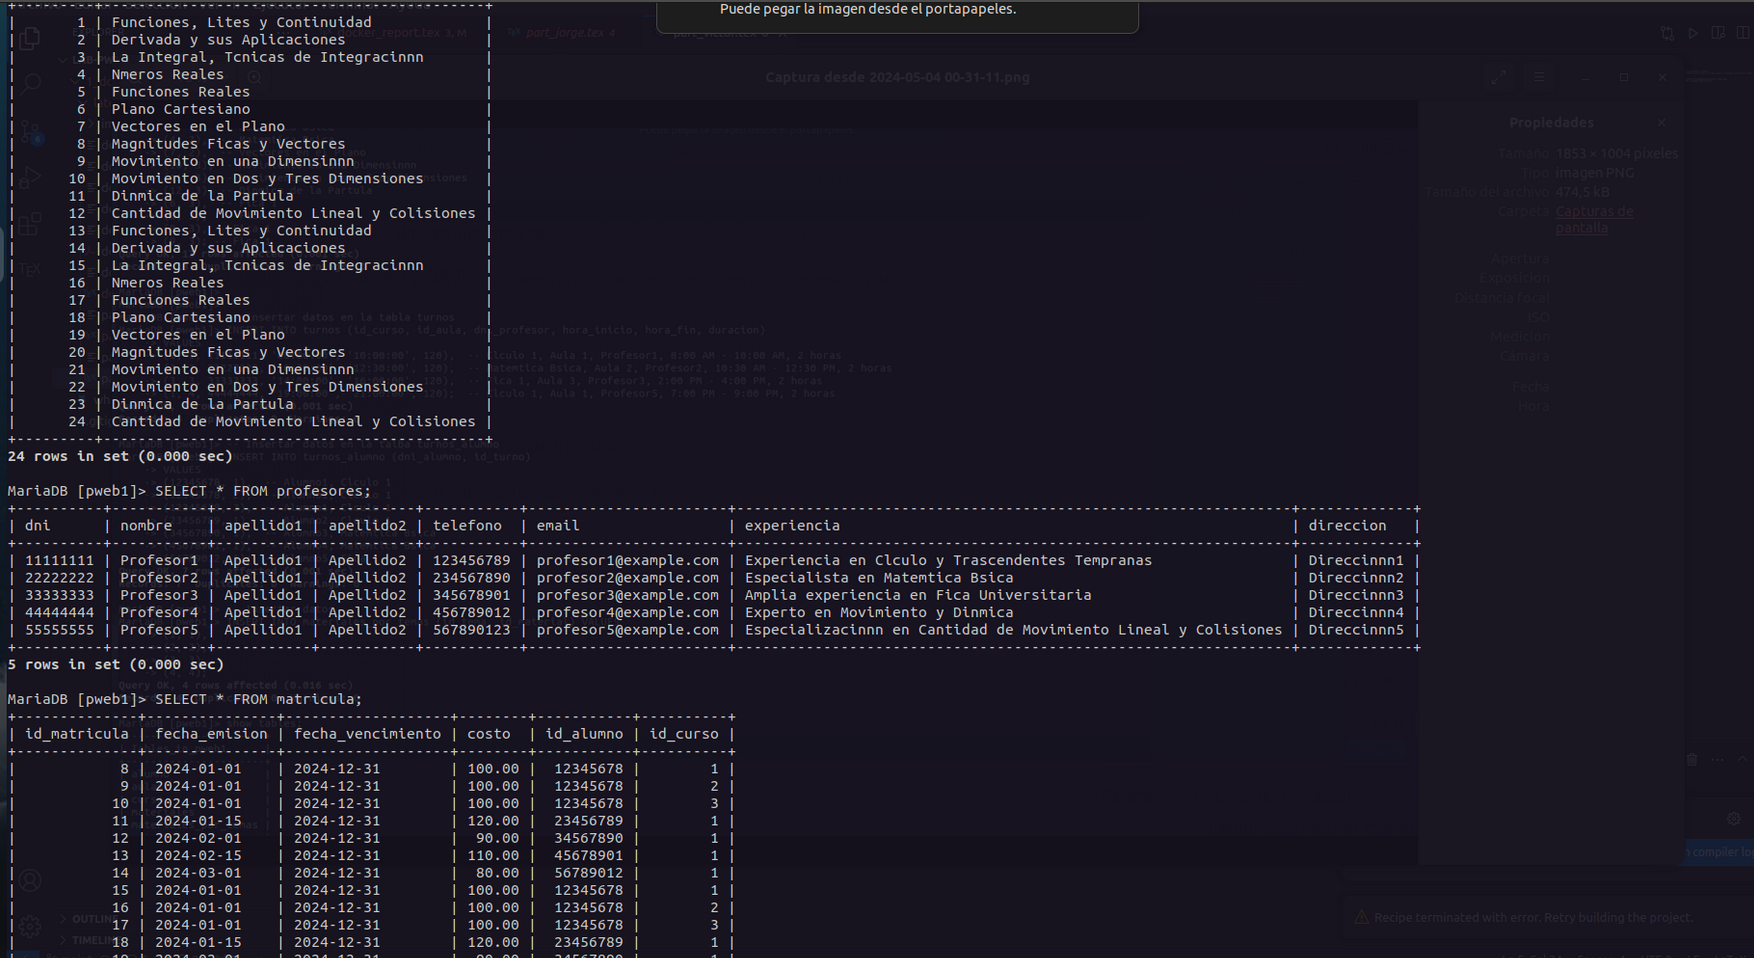
\includegraphics[width=1.0\textwidth]{img/Viendo_Datos_3.png}
  \caption{Visualizamos las tablas de la Base de Datos}
\end{figure}
\begin{figure}[H]
  \centering
  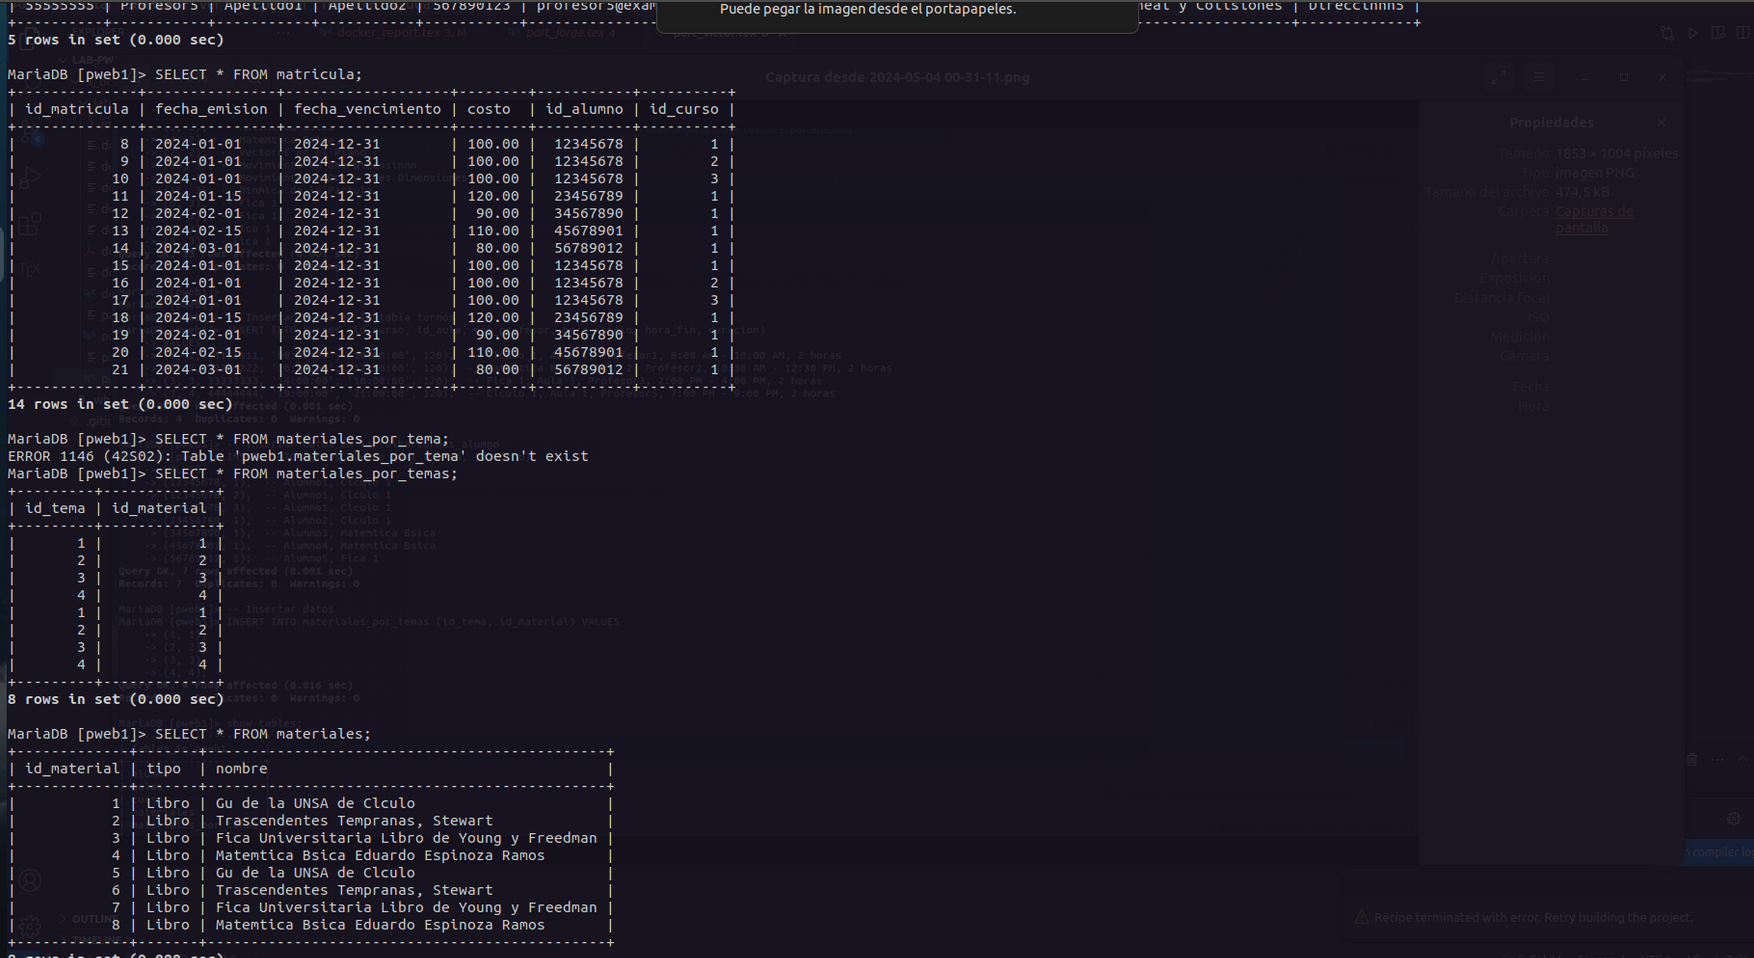
\includegraphics[width=1.0\textwidth]{img/Viendo_Datos_2.png}
  \caption{Visualizamos las tablas de la Base de Datos}
\end{figure}
\begin{figure}[H]
  \centering
  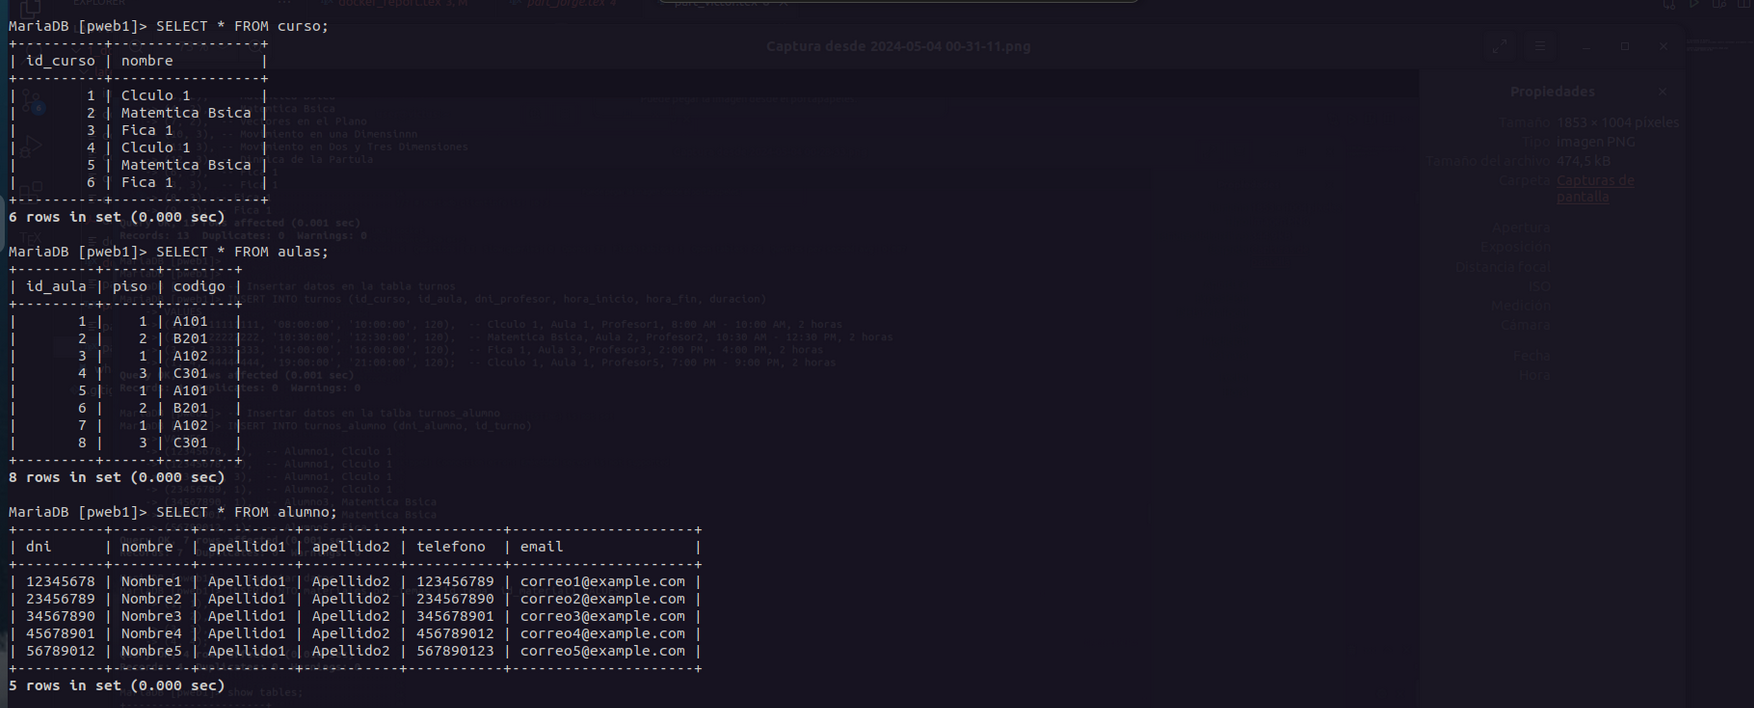
\includegraphics[width=1.0\textwidth]{img/Viendo_Datos_1.png}
  \caption{Visualizamos las tablas de la Base de Datos}
\end{figure}

Creamos el usuario pw2 y contraseña 12345678 el cual sera con el que podamos entrara a la base de datos y tenga los permisos necesarios
\begin{figure}[H]
  \centering
  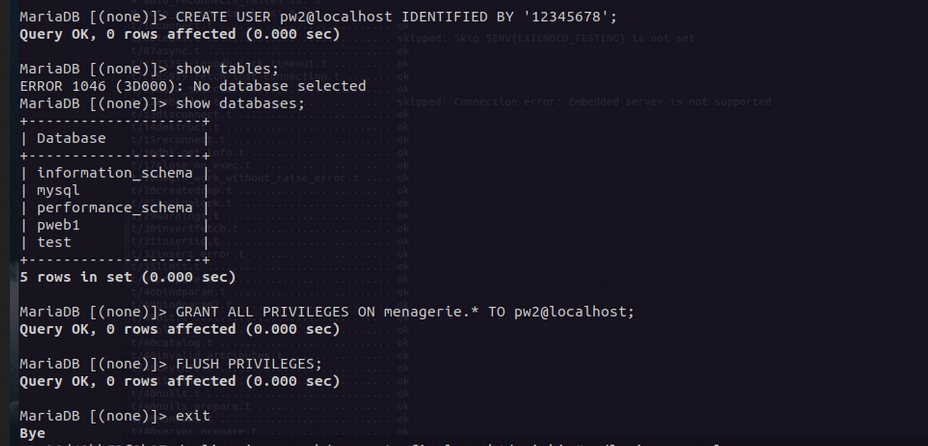
\includegraphics[width=1.0\textwidth]{img/Creamos_usuario_MariaDB.png}
  \caption{Creamos el ususario pw2 y su contraseña}
\end{figure}
\begin{figure}[H]
  \centering
  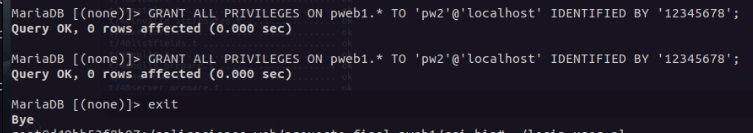
\includegraphics[width=1.0\textwidth]{img/Dando_Permisos.png}
  \caption{Al usuario pw2 le damos los permisos para la base de datos pweb1}
\end{figure}

Entonces para ya finzalizar tendriamos que probar el funcionamiento de nuestro proyecto en el servidor para entonces primero cambiamos de dominio a nuestro ip
de contenedor y lo referenciamos a uno mas centrado por lo que nosotros le pondremos academiapiensa.con para esto cambiamos el .conf del directorio de nuestro
proyecto y tambien en nuestra maquina local que no es docker tambien configuramos el /etc/hosts/ al ip del contenedor contal que cuando ingresemos en este dominio 
visualizaremos el proyecto 
\begin{figure}[H]
  \centering
  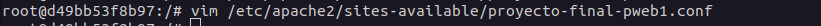
\includegraphics[width=1.0\textwidth]{img/Ingresando.png}
  \caption{Entrando en la configuracion del contenedor para el ServerName}
\end{figure}
\begin{figure}[H]
  \centering
  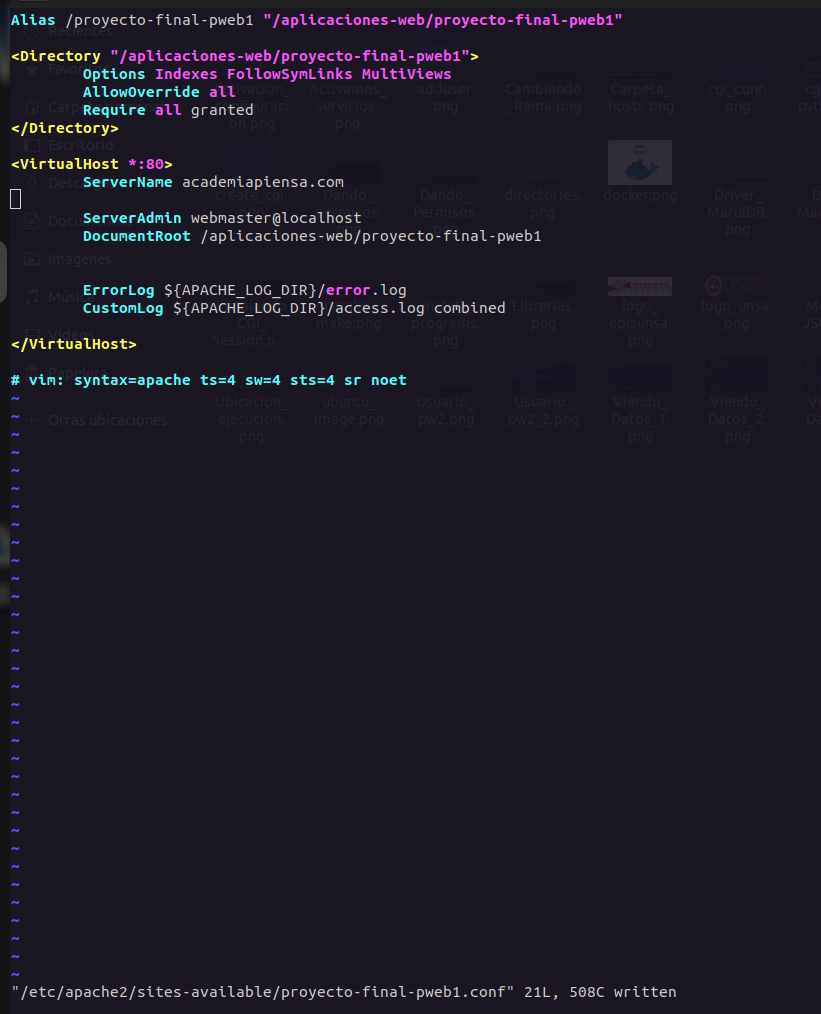
\includegraphics[width=1.0\textwidth]{img/Configuracion_ServerName.png}
  \caption{Configurando el directorio para Apache}
\end{figure}
\begin{figure}[H]
  \centering
  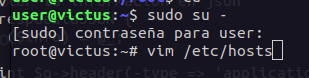
\includegraphics[width=1.0\textwidth]{img/Ingresando_Maq_Local.png}
  \caption{Entrando en la configuracion maquina local para el ServerName}
\end{figure}
\begin{figure}[H]
  \centering
  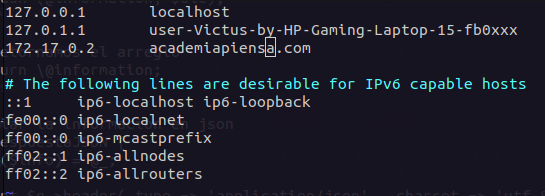
\includegraphics[width=1.0\textwidth]{img/Conf_Maq_Local.png}
  \caption{Hacemos las referencias}
\end{figure}

Finalizamos con la presentacion de nuestro proyecto con capturas de pantalla y tambien el url del dominio 
\begin{figure}[H]
  \centering
  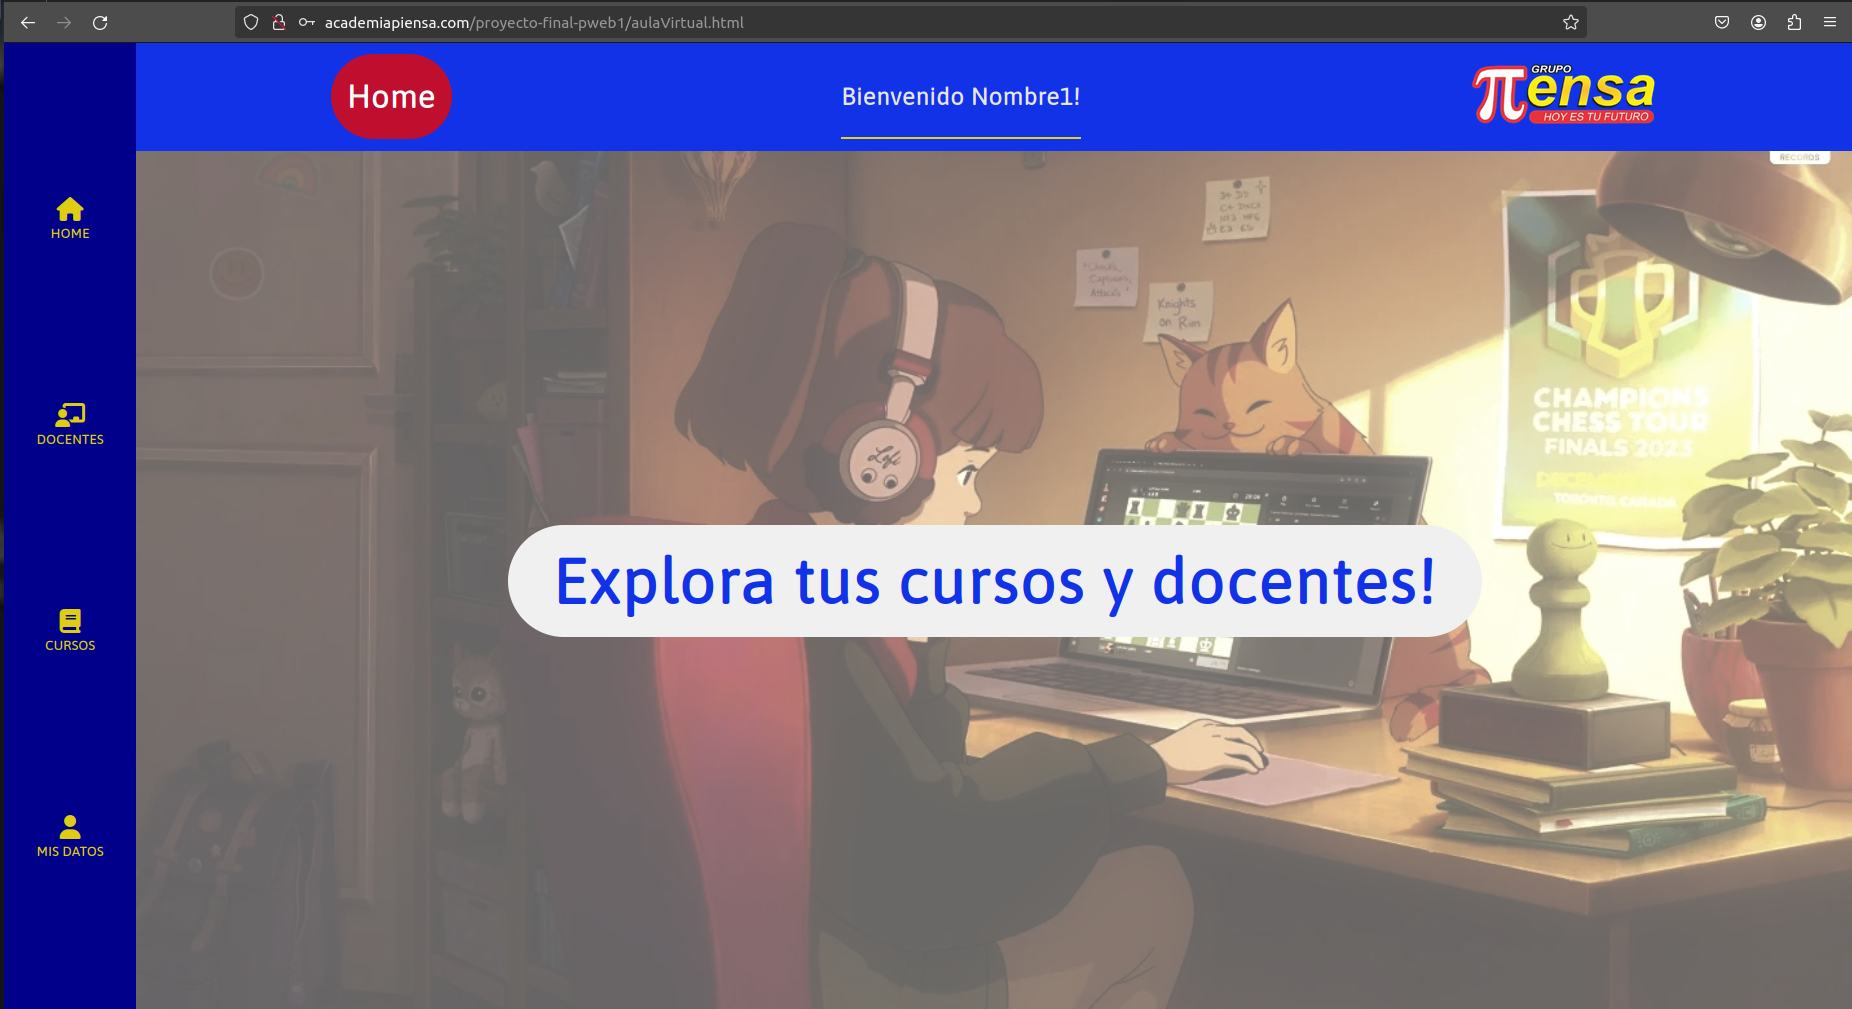
\includegraphics[width=1.0\textwidth]{img/AulaVirtual.png}
  \caption{Pagina Web en funcionamiento con el dominio academiapiensa.com}
\end{figure}
\begin{figure}[H]
  \centering
  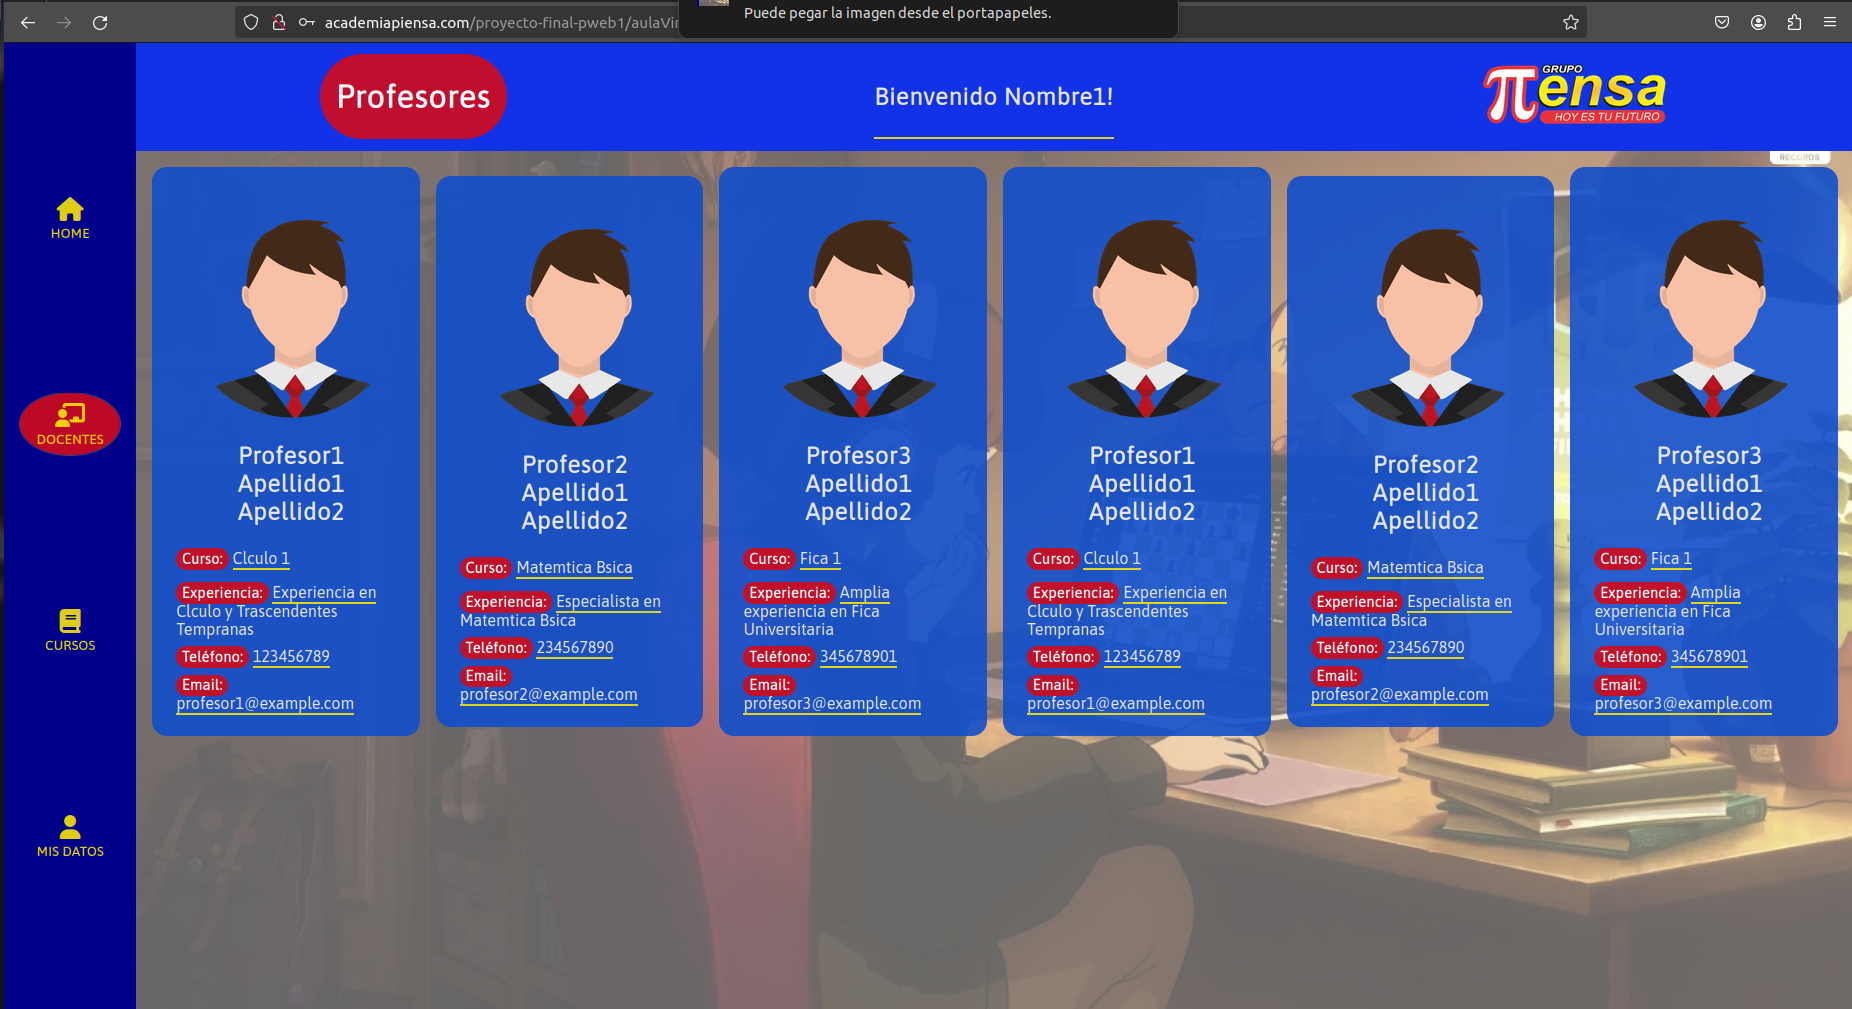
\includegraphics[width=1.0\textwidth]{img/AulaVirtual2.png}
  \caption{Pagina Web en funcionamiento con el dominio academiapiensa.com}
\end{figure}
\begin{figure}[H]
  \centering
  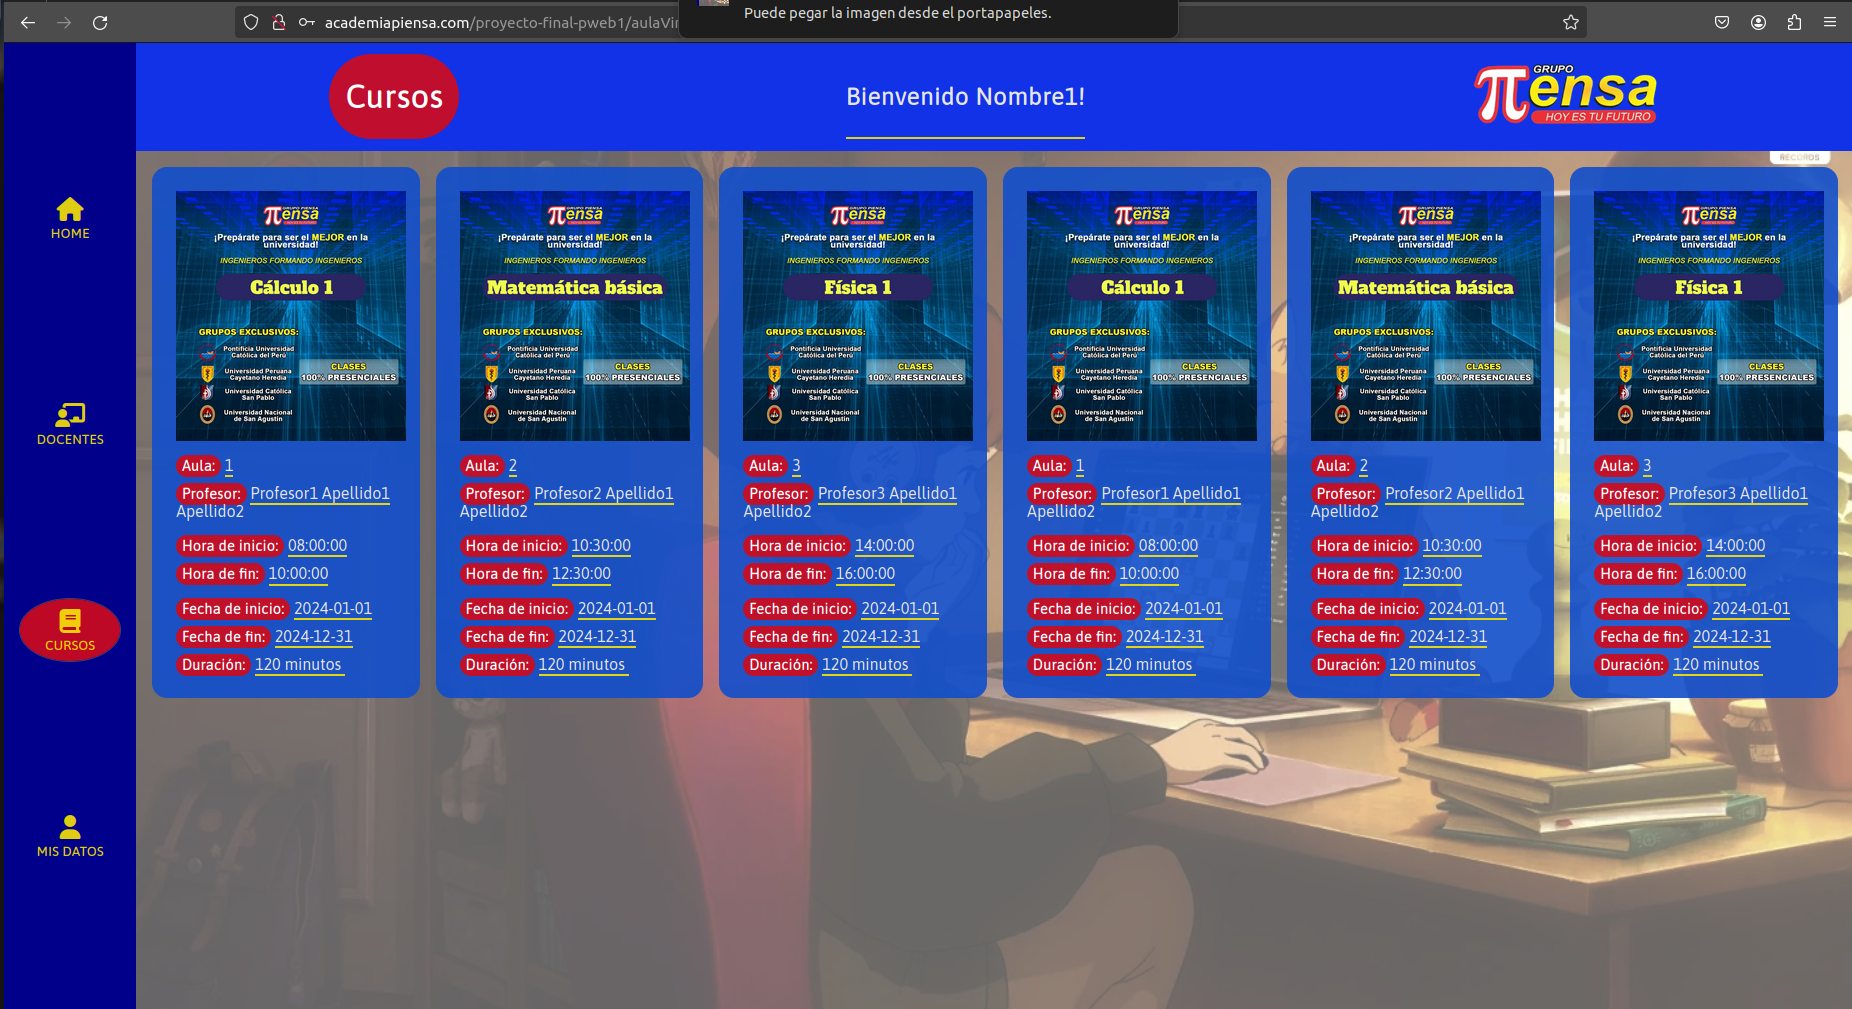
\includegraphics[width=1.0\textwidth]{img/AulaVirtual3.png}
  \caption{Pagina Web en funcionamiento con el dominio academiapiensa.com}
\end{figure}
\begin{figure}[H]
  \centering
  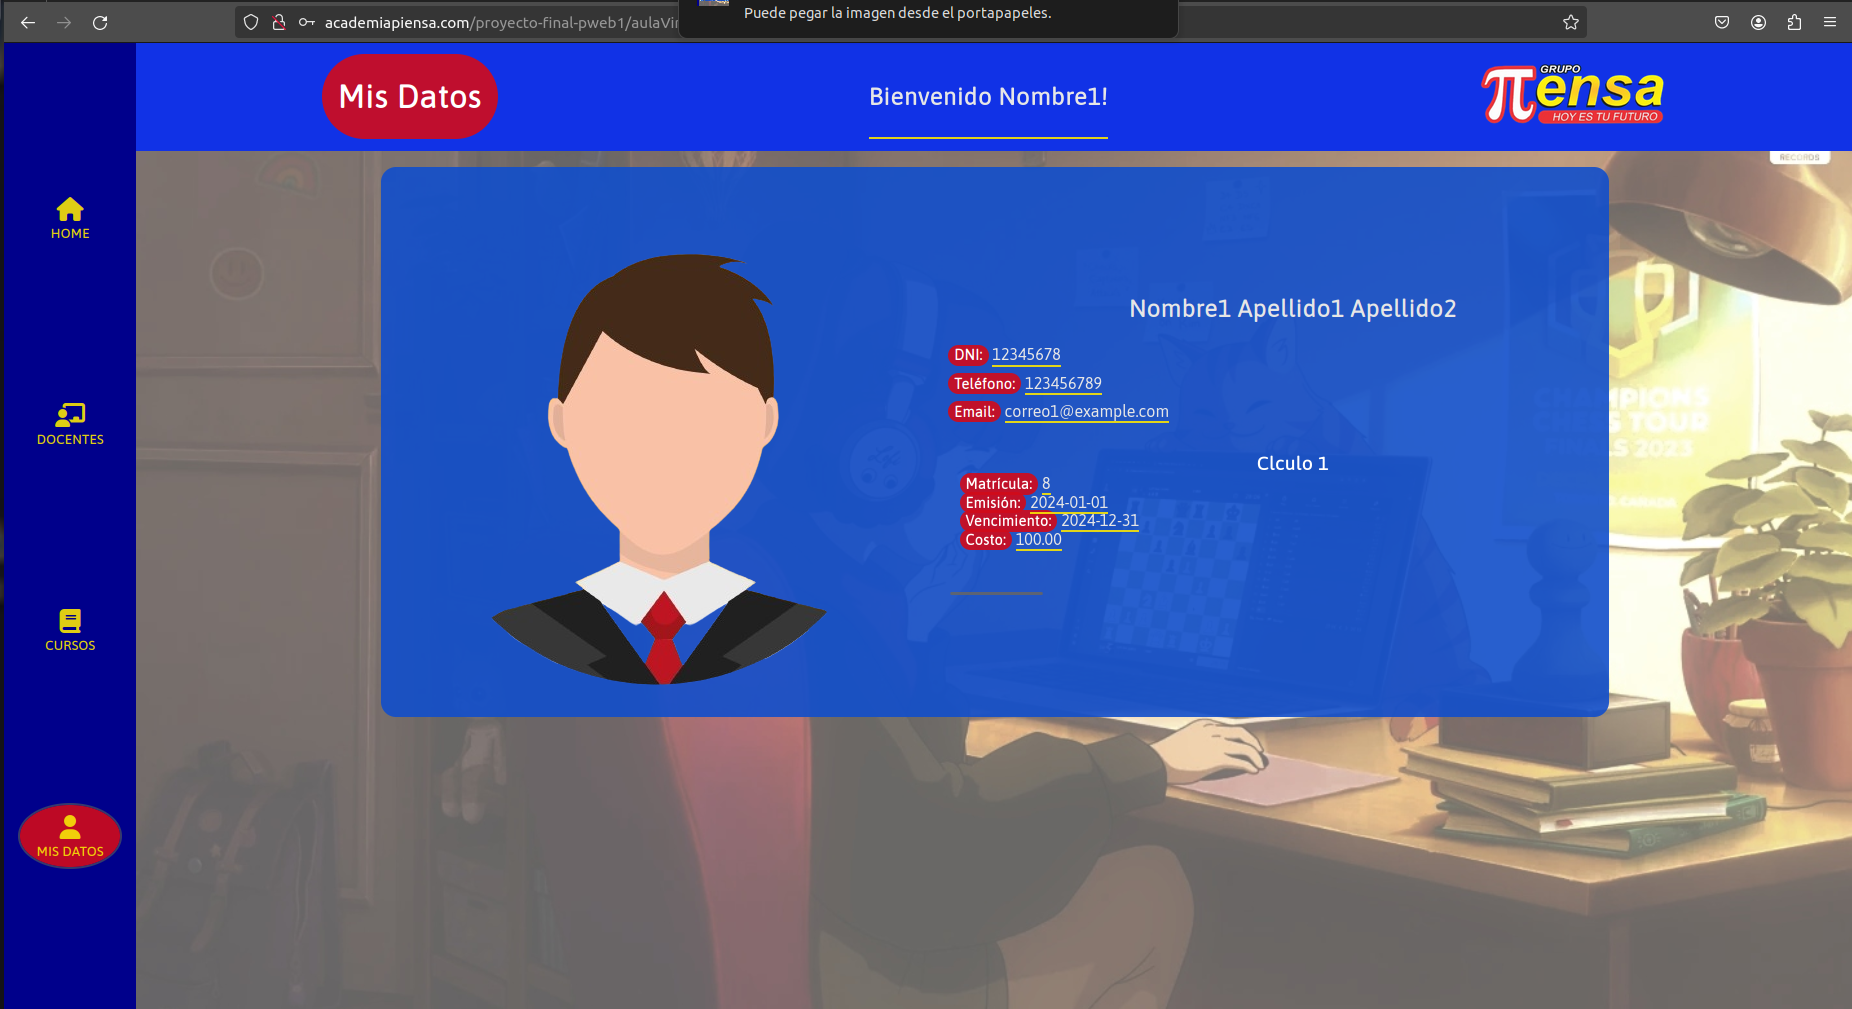
\includegraphics[width=1.0\textwidth]{img/AulaVirtual4.png}
  \caption{Pagina Web en funcionamiento con el dominio academiapiensa.com}
\end{figure}
\begin{figure}[H]
  \centering
  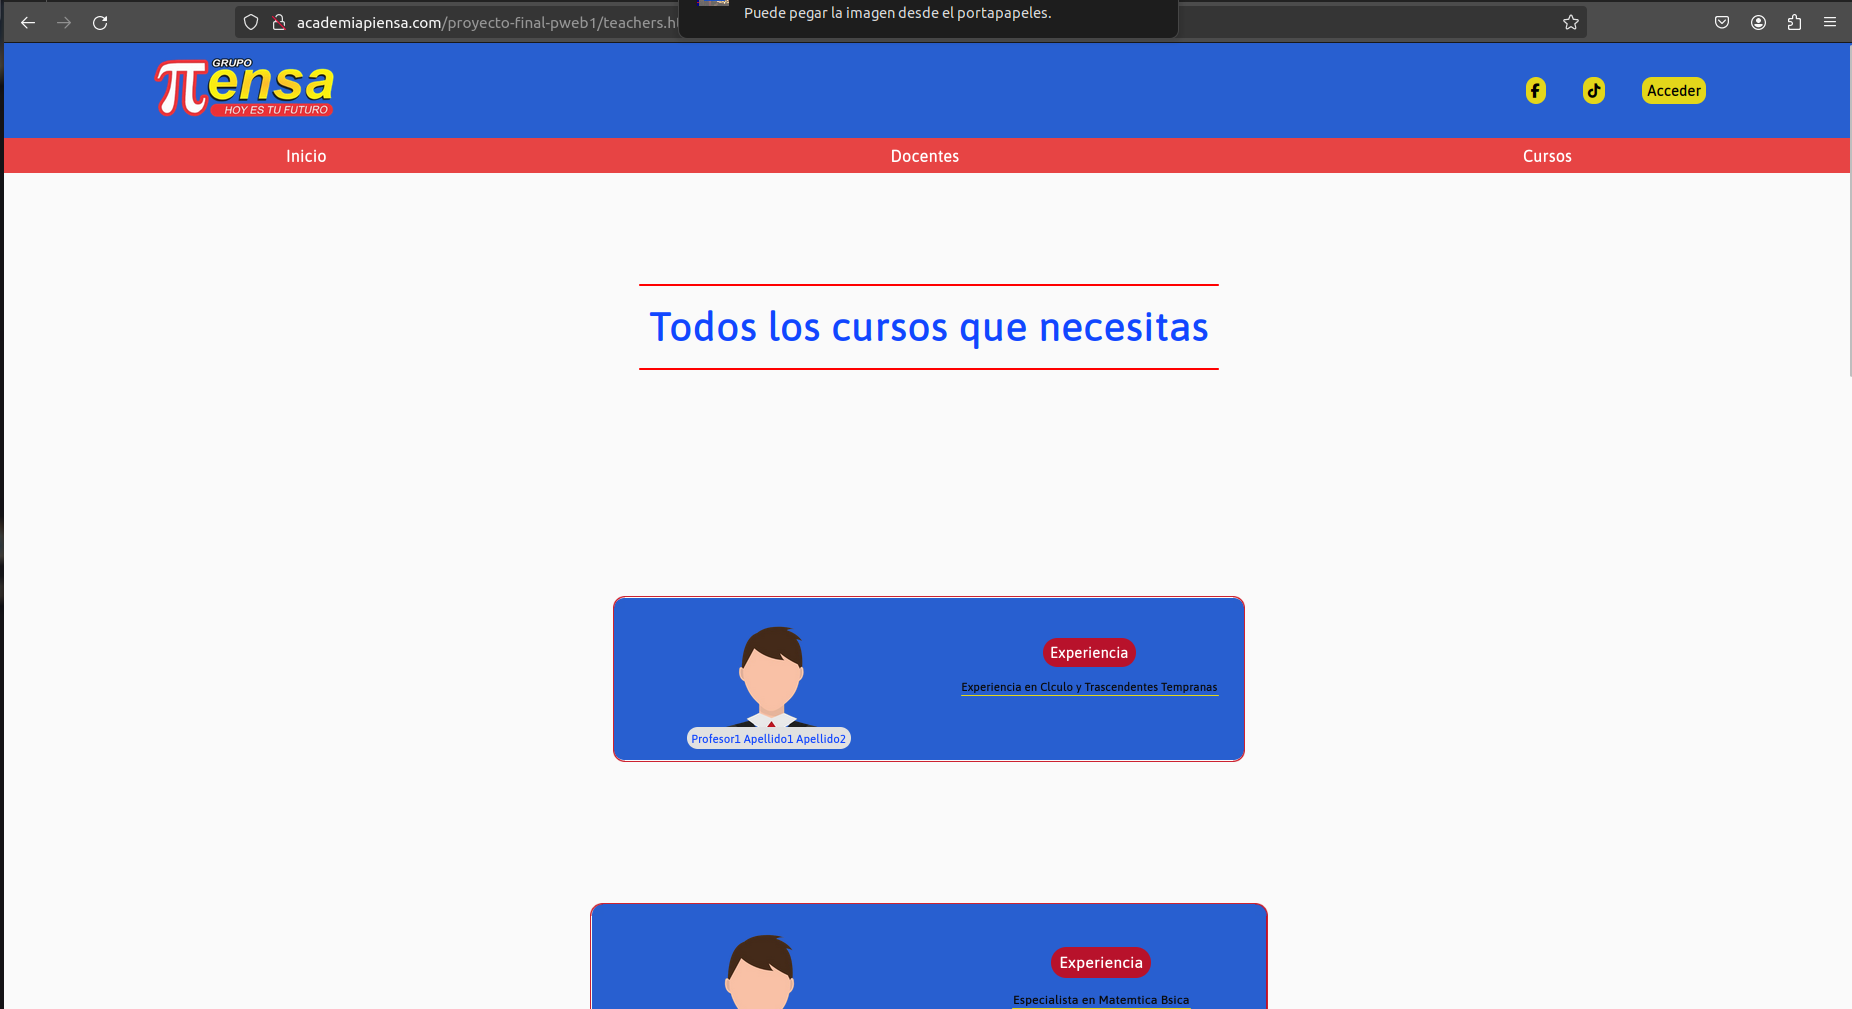
\includegraphics[width=1.0\textwidth]{img/Profesores.png}
  \caption{Pagina Web en funcionamiento con el dominio academiapiensa.com}
\end{figure}
\begin{figure}[H]
  \centering
  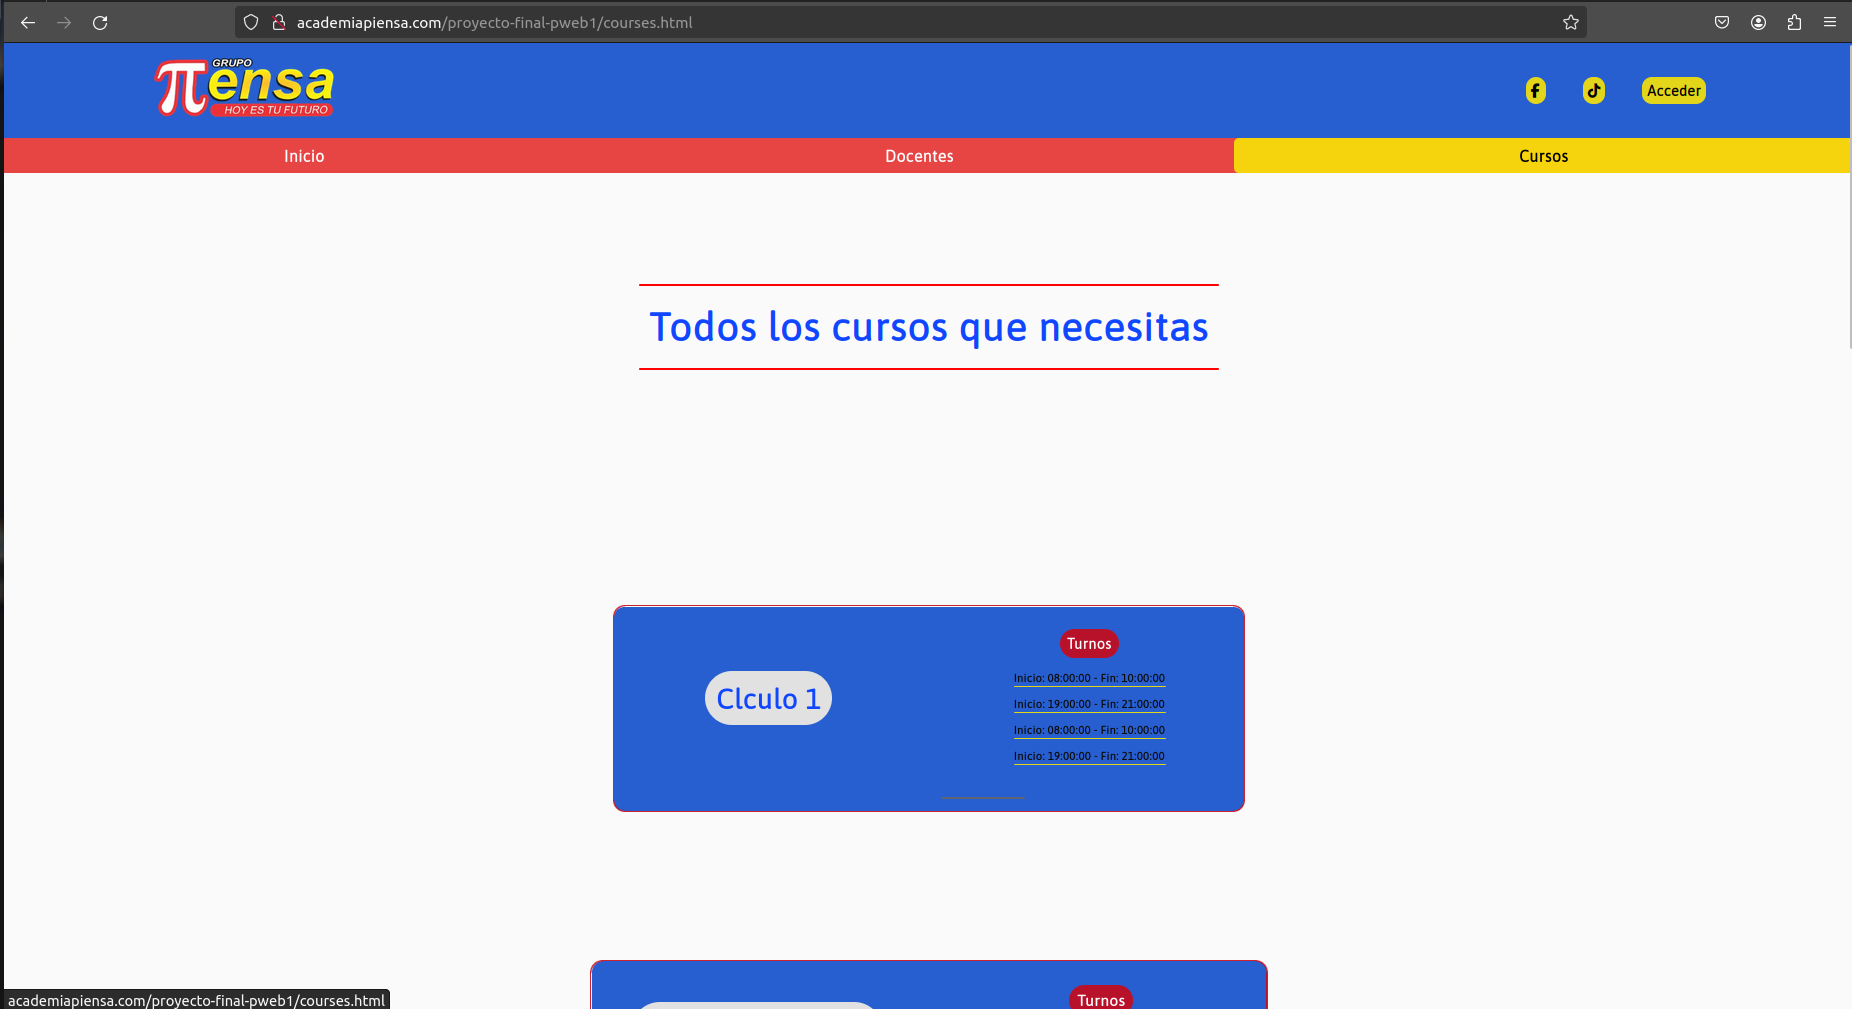
\includegraphics[width=1.0\textwidth]{img/Cursos.png}
  \caption{Pagina Web en funcionamiento con el dominio academiapiensa.com}
\end{figure}
\begin{verbatim}
  URL del video:
\end{verbatim}